\section[Реализация программного модуля]{%
  РЕАЛИЗАЦИЯ ПРОГРАММНОГО МОДУЛЯ
}\label{sec:implementation}

\subsection{Выбор программных средств реализации}

Мобильная платформа Android в значительной мере
определяет набор средств разработки. Большинство Android-приложений
разрабатываются на языке программирования Java. Программирование
приложения производится c помощью специализированной
интегрированной среды разработки Android Studio
с использованием Android Software Developement Kit (SDK)
и Native Developement Kit (NDK).

Существует некоторая свобода выбора в отношении используемой СУБД.
Следует отметить, что системы управления базами данных,
используемые на мобильных платформах, существенно отличаются
от традиционных решений.
Это вызвано тем, что работа мобильных баз данных производится в
иных условиях, характеризующися следующими особенностями:
\begin{itemize}
  \item малый рабочий объем данных;
  \item низкая плотность потока запросов обработки данных;
  \item отсутствие необходимости обработки параллельных транзакций;
  \item программный интерфейс приложения-клиента заранее известен.
\end{itemize}

Первые три условия вызваны тем, что СУБД обрабатывает запросы
лишь одного клиента --- пользователя приложения.
Последнее условие вызвано тем, что программный интерфейс мобильных
приложений для платформы Android известен по определению (Java VM).

С другой стороны, мобильные платформы выдвигают ряд
дополнительных требований к СУБД.
Во-первых, работа базы данных должна производиться в рамках
процесса клиентского приложения, поскольку Android не гаратирует
неприкосновенности пользовательских процессов, то есть они могут быть
приостановлены или завершены в любой момент времени.
Во-вторых, механизм хранения данных должен быть централизованным,
компактным и переносимым. Это требование накладывает
известные ограничения на используемые структуры данных
и алгоритмы их обработки.

Существует несколько популярных СУБД для мобильных устройств.
По умолчанию Android предоставляет возможность хранения
данных с использованием SQLite --- малой реляционной СУБД,
используемой также и на персональных компьютерах.
Характерными особенностями данной СУБД являются поддержка SQL,
хранение данных в едином файле и отсутствие необходимости конфигурирования.
Кроме этого, существует несколько альтернативных СУБД~\cite{mobile_db}:
Cupboard, BerkeleyDB, Couchbase Lite, LevelDB, Realm, UnQLite.

В разрабатываемом приложении используется СУБД Realm~\cite{realm_official}.
Выбор обусловлен несколькими причинами.
Во-первых, Realm является объектно-ориентированной СУБД,
что избавляет от необходимости написания слоя трансляции объектов Java
в сущности реляционной БД.
Во-вторых, он имеет более высокую производительность по сравнению с SQLite.
В-третьих, данный проект активно развивается, имеет подробную документацию,
является открытым и бесплатным.
Кроме этого, приложение использует библиотеки OpenCV~\cite{opencv}
(для обработки и распознавания изображений),
Appcompat (для реализации рекомендаций Material Design на старых версиях платформы Android)
и JUnit (для организации тестирования приложения).

\subsection{Реализация подсистемы хранения данных}
\label{subsec:implementation_db}

Поскольку Realm является объектно-ориентированной СУБД,
сущности модели данных, разработанной в подразделе~\ref{subsec:design_information},
находят свое отражение в соответствующих им классах Java.
При этом к классам модели данных предъявляются следующие дополнительные требования:
\begin{itemize}
  \item данные классы должны быть унаследованы от \textit{RealmObject};
  \item каждый класс должен иметь публичный конструктор по умолчанию (без параметров);
  \item набор типов хранимых данных ограничен набором базовых типов,
    а также другими классами модели данных.
\end{itemize}

Realm поддерживает хранение следующих базовых типов данных:
\textit{boolean}, \textit{byte}, \textit{short}, \textit{ìnt},
\textit{long}, \textit{float}, \textit{double}, \textit{String},
\textit{Date} и \textit{byte[]}.
К сожалению, хранение данных типа \textit{Currency}, а также
\textit{Enum} на данный момент не поддерживается.
Поддержка отношений вида 1:1 может быть реализована
путем хранения одиночных ссылок на другие объекты Realm внутри данного.
Поддержка отношений вида 1:M, M:M
реализована через хранение списков ссылок (\textit{RealmList}).

Доступ к подсистеме базы данных осуществляется через класс
\textit{DBManager}. Данный класс представляет собой \textit{синглтон},
выполняющий инициализацию и контроль доступа к объектам Realm
со стороны подсистемы обработки данных.
Для работы с данными предусмотрены статические классы
\textit{AccountOperations}, \textit{CategoryOperations}
и \textit{BalanceChangeOperations}, предоставляющие
программный интерфейс для создания, чтения, обновления и
удаления соответствующих объектов Realm.

На рисунке~\ref{lst:implementation_db_account} в качестве примера
представлен класс \textit{Account}, соответствующий сущности <<УчетнаяЗапись>>
исходной модели данных.

\lstinputlisting[
    caption=Пример класса модели данных,
    language={Java},
    label=lst:implementation_db_account,
]{lst/implementation_db_account.lst}

Данный класс является публичным, унаследованным от класса \textit{RealmObject}.
Он содержит набор приватных полей данных: название, индекс, код валюты,
а также список связанных объектов \textit{BalanceChange},
соответствующих изменениям баланса.
Кроме этого, он содержит публичное строковое поле, соответствующее
названию поля индекса и используемое для сортировки.
Большинство методов класса выполняют чтение/модификацию
полей объекта; метод \textit{getBalanceChanges} возвращает ссылку на
список связанных изменений баланса,
а метод \textit{getTotalAmount} использует встроенную
агрегатную функцию для получения суммы значений данных изменений.
Полный исходный код реализации модели данных представлен в приложении~А.

\subsection{Реализация подсистемы компьютерного зрения}
\label{subsec:implementation_cv}

Подсистема компьютерного зрения инкапсулирует детали реализации
разработанного алгоритма оптического распознавания данных,
описанного в подразделе~\ref{ssec:design_algorithm}.
Ввиду высокой вычислительной сложности алгоритма
он разделен на две части:
построение модели классификатора,
производимое на персональном компьютере разработчика и
собственно распознавание данных,
производимое на целевом мобильном устройстве.
На рисунках~\ref{fig:implementation_cv_trainer}
и~\ref{fig:implementation_cv_recognizer} приведены схемы работы
описанных частей алгоритма.
Файлы тренировочных изображений и из классов содержат
данные базы рукописных цифр MNIST.
Модель обученного классификатора хранится в файле формата XML
и является частью мобильного приложения.
Реализация алгоритмов подсистемы компьютерного зрения
выполнена на языке программирования C++.
Взаимодействие кода, написанного на языке программирования Java,
с кодом на C++ организовано посредством стандартизированного
программного интерфейса \textit{JNI}~\cite{spec_jni}.
Данный подход используется для получения максимальной скорости
распознавания данных на мобильном устройстве.
Общие части кодовой базы, написанной на C++, выделены в статические библиотеки.

\begin{figure}[h!]
  \centering
  \fcolorbox{gray}{white}{
    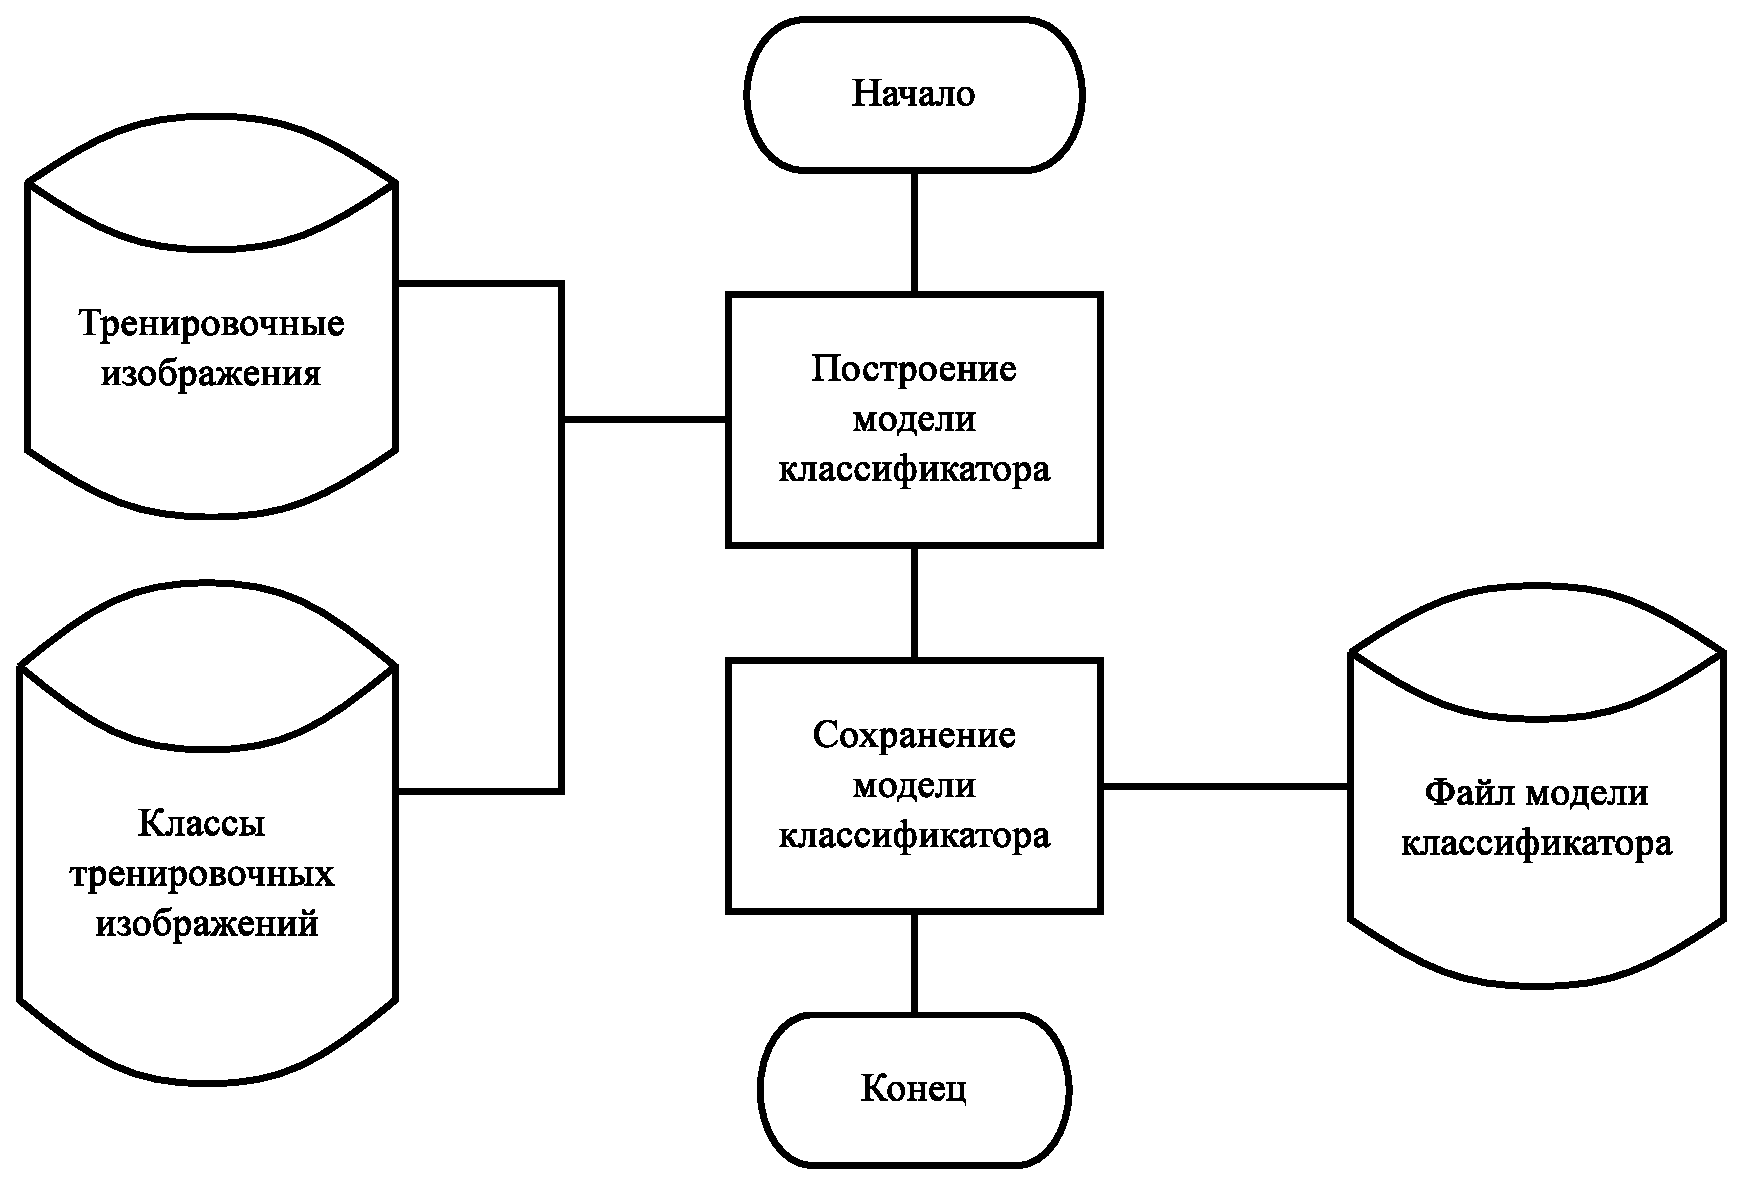
\includegraphics[width=140mm]{fig/implementation_cv_trainer.eps}
  }
  \caption{Схема построения модели классификатора}
  \label{fig:implementation_cv_trainer}
\end{figure}

\begin{figure}[h!]
  \centering
  \fcolorbox{gray}{white}{
    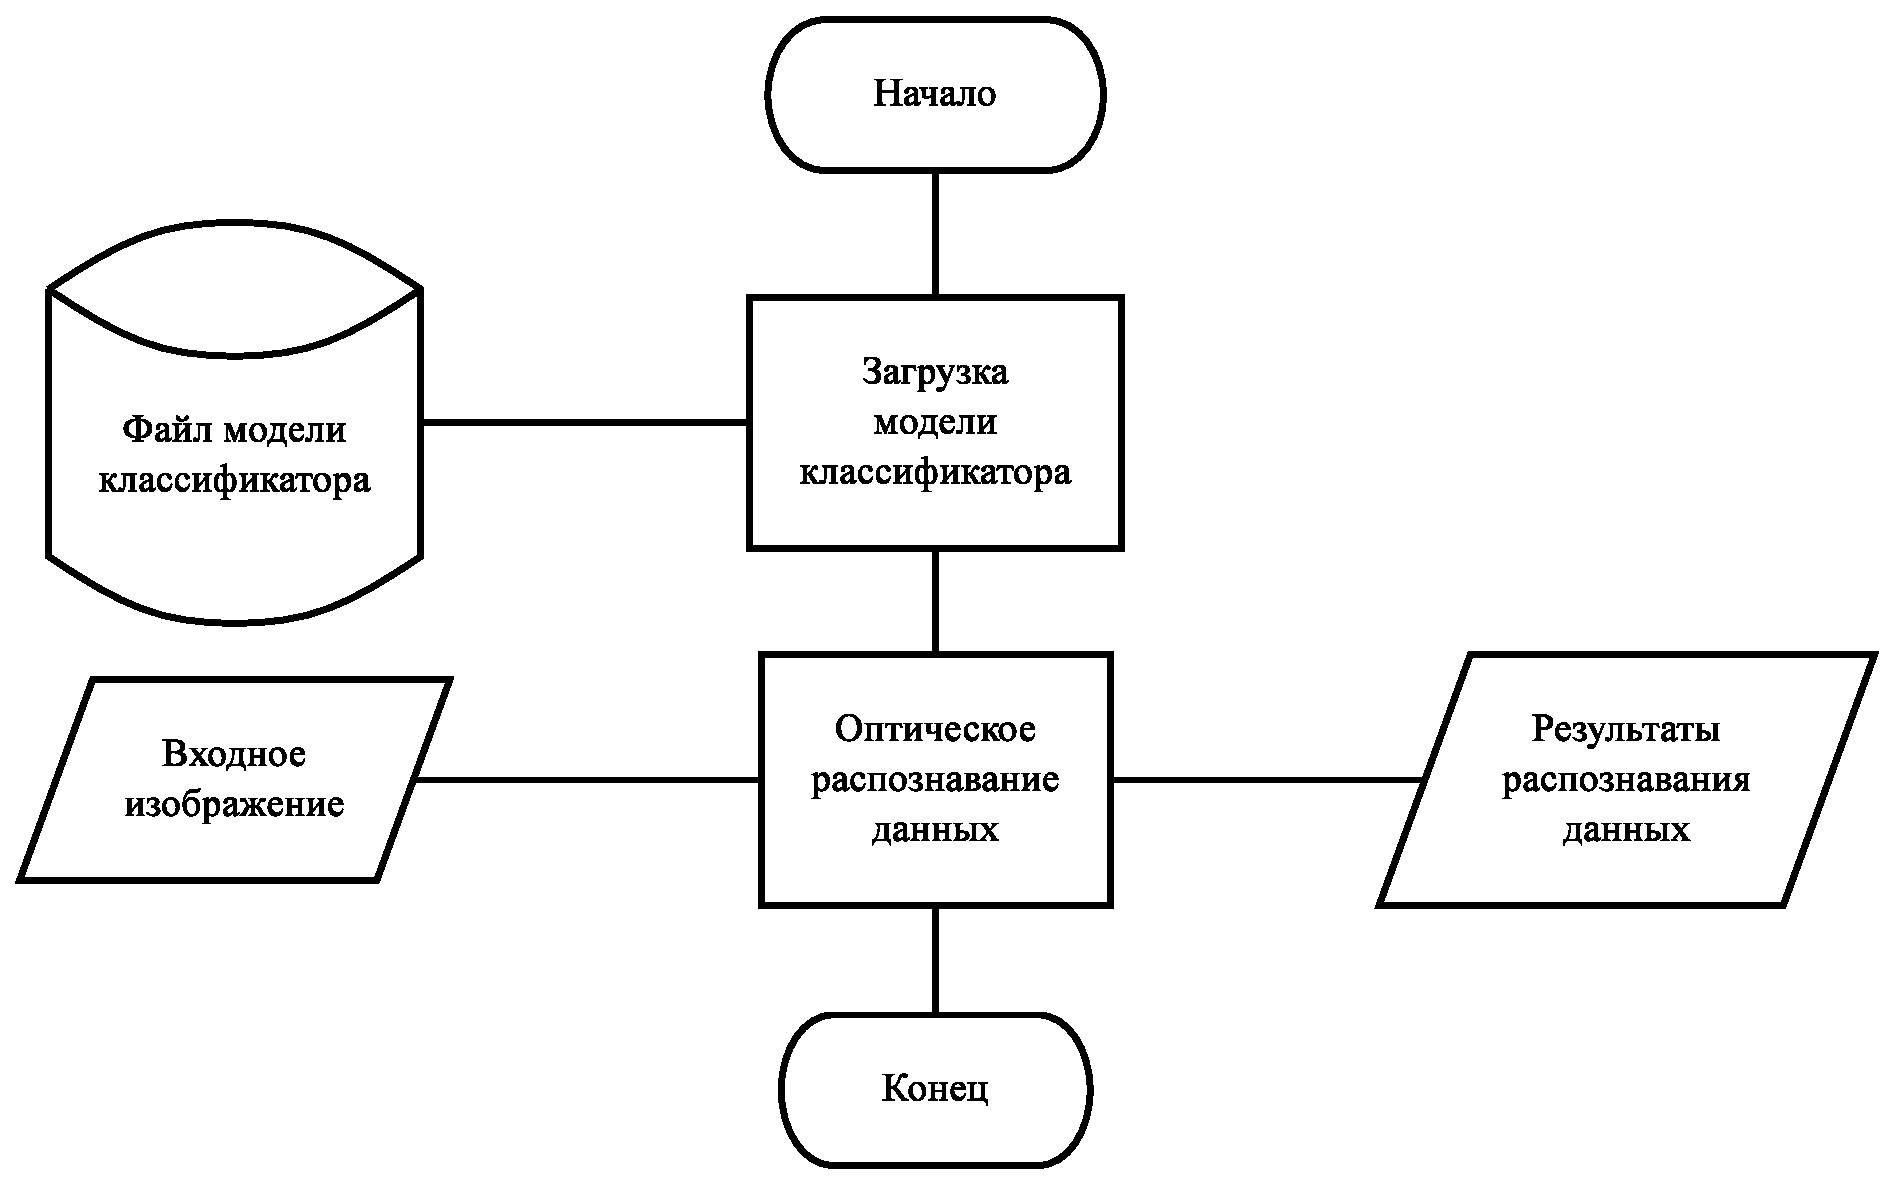
\includegraphics[width=140mm]{fig/implementation_cv_recognizer.eps}
  }
  \caption{Схема распознавания изображения}
  \label{fig:implementation_cv_recognizer}
\end{figure}

На рисунке~\ref{lst:implementation_cv_trainer} представлен фрагмент
исходного кода программы построения модели классификатора,
иллюстрирующий сущность её работы.
Данная консольная программа принимает следующие аргументы командной
строки: путь к изображениям для тренировки модели,
путь к классам тренировочных изображений и
путь к файлу для сохранения полученной модели (строки 5--7).
С помощью объекта класса \textit{MnistLoader} производится загрузка
тренировочных данных из файлов базы MNIST (строки 9--12).
С помощью объекта класса \textit{HOGDescriptor}, предоставляемого
библиотекой OpenCV, производится расчет HOG-дескрипторов для
входных данных (строки 14--19). Параметры конструктора данного объекта
соответствуют параметрам алгоритма вычисления дескриптора
и пропорциональны размерам исходных изображений.
Далее производится приведение множества полученных дескрипторов
к совместимой с классификатором форме:
дескрипторы объединяются в матрицу, ширина которой
соответствует числу элементов дескриптора, а высота ---
числу самих дескрипторов (строки 20--29).
Множество дескрипторов и соответствующих им классов используется
для обучения SVM-модели классификатора, предоставляемого библиотекой
OpenCV (строки 31--37).
Полученная модель записывается в файл (строка 38).
Полный исходный код программы обучения модели классификации представлен
в приложении Б.

\lstinputlisting[
    caption=Построение модели классификатора,
    language={C++},
    label=lst:implementation_cv_trainer,
]{lst/implementation_cv_trainer.lst}

Подсистема компьютерного зрения состоит из двух частей.
Часть подсистемы, написанная на языке
программирования Java, расположена в пакете \textit{cv}. Посредством
интерфейса JNI она взаимодействует с частью подсистемы, написанной на C++.
Исходный код подпрограммы распознавания изображений, приведенный в приложении В,
подобен коду программы построения модели классификации.
Основные его отличия сводятся к тому,
что в ней используется обученная ранее модель классификации и
выполняется предварительная обработка входного изображения.

Библиотека OpenCV предоставляет удобный интерфейс работы с камерой
мобильного устройства в виде компонента пользовательского интерфейса
\textit{JavaCameraView}.
Данный класс предоставляет доступ своим наследникам
к изображениям фотокамеры, позволяя им выполнять
необходимую обработку, как показано на рисунке~\ref{lst:implementation_cv_camera}.

\lstinputlisting[
    caption=Организация доступа к изображением фотокамеры,
    language={Java},
    label=lst:implementation_cv_camera,
]{lst/implementation_cv_camera.lst}

Здесь аргументом метода \textit{onCameraFrame} является
изображение, полученное с фотокамеры, а возвращаемым значением ---
результат его обработки. В приведенном примере производится выделение
зоны интереса фиксированного размера и его начальная обработка.
На рисунке~\ref{fig:implementation_cv_recognition} представлен
пример работы алгоритма оптического распознавания данных.

\begin{figure}[h!]
  \centering
  \fcolorbox{gray}{white}{
    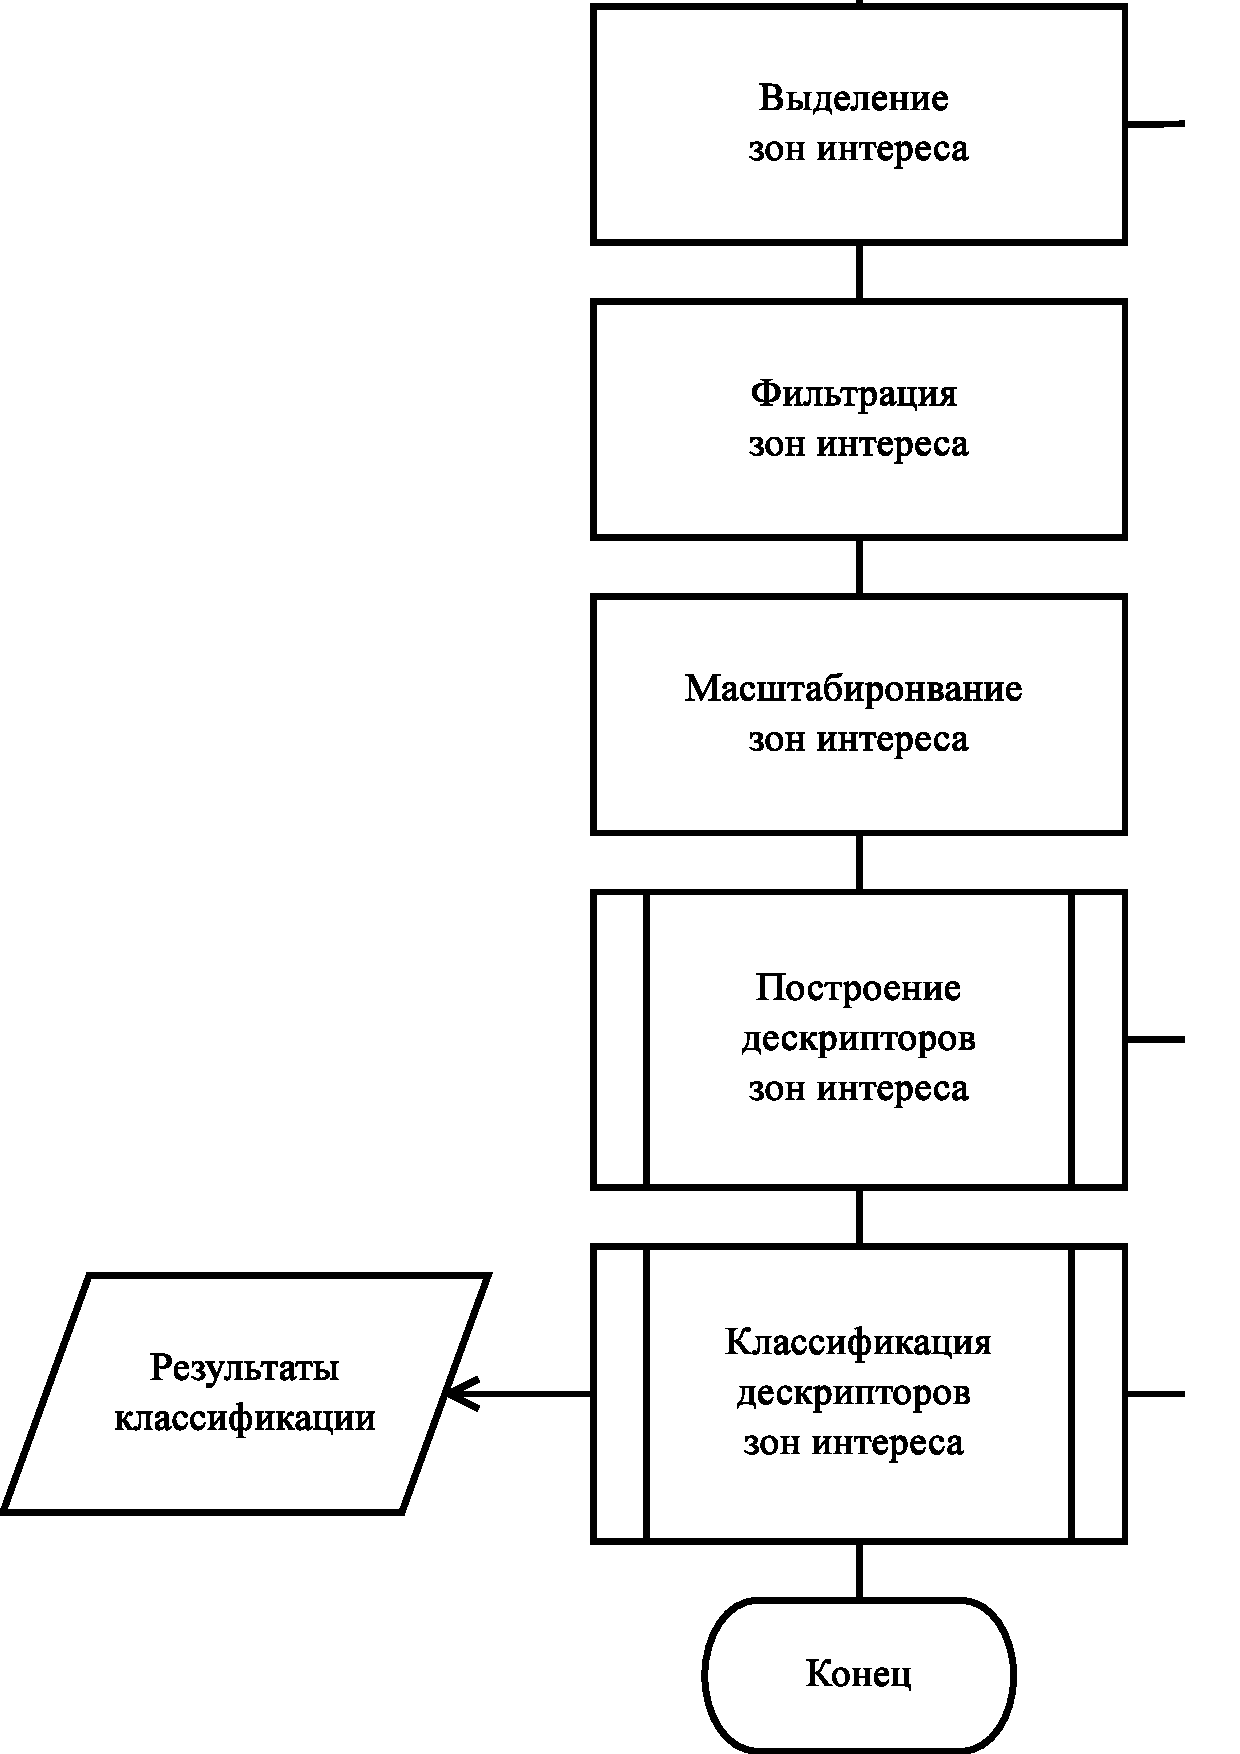
\includegraphics[width=90mm]{fig/implementation_cv_recognition.png}
  }
  \caption{Пример работы алгоритма \\ оптического распознавания данных}
  \label{fig:implementation_cv_recognition}
\end{figure}

В верхней части показано исходное изображение;
далее --- результат применения фильтра предварительной обработки,
затем --- выделенные зоны интереса, и, наконец, конечный результат распознавания.


\subsection{Реализация пользовательского интерфейса}
\label{subsec:implementation_ui}

Организация пользовательского интерфейса мобильных приложений
платформы Android базируется на трех классах:
\textit{Activity}, \textit{Fragment} и \textit{View}.
Класс \textit{Activity} (экран) соответствует отдельному экрану приложения.
Класс \textit{Fragment} (фрагмент) соответствует относительно самостоятельной части
экрана приложения.
Экраны и фрагменты содержат множество экземпляров класса \textit{View},
соответствующего базовым элементам интерфейса --- полям, кнопкам, и~т.~д.
Взаимосвязь этих классов приведена на рисунке~\ref{fig:implementation_ui_hierarchy}.

\begin{figure}[h!]
  \centering
  \fcolorbox{gray}{white}{
    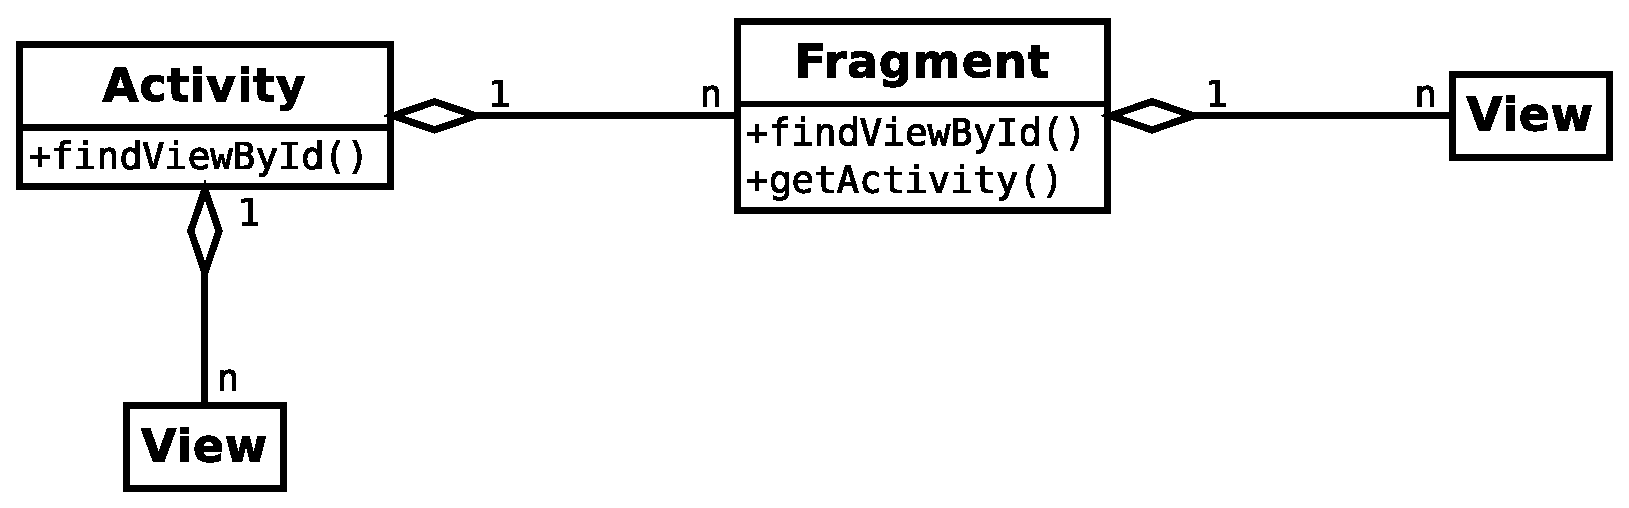
\includegraphics[width=140mm]{fig/implementation_ui_hierarchy.eps}
  }
  \caption{Организация базовых классов \\ пользовательского интерфейса Android}
  \label{fig:implementation_ui_hierarchy}
\end{figure}

Введение понятия фрагмента обусловлено необходимостью унификации
механизма поддержки пользовательского интерфейса для устройств с различными
размерами дисплея. Так, например, на устройствах с большим размером дисплея
один экран приложения может содержать несколько фрагментов, а на малом ---
каждый фрагмент будет находиться в отдельном экране.
Связь между экраном и фрагментом осуществляется следующим образом:
экраны хранят ссылки на созданные ими фрагменты,
а фрагменты могут получить ссылку на родительские экраны путем
вызова метода \textit{getActivity}.
Для получения ссылки на требуемый объект класса \textit{View}
используется метод \textit{findViewById}.

Платформа Android управляет экранами и фрагментами путем вызова ряда методов,
определенных в базовых классах. Совокупность данных методов образует
жизненный цикл элемента интерфейса. Каждый из них принимает
специльный аргумент типа \textit{Bundle}, позволяющий передавать
аргументы примитивных типов, а также сохранять и восстанавливать
собственное состояние.
На рисунке~\ref{fig:implementation_ui_lifecycle_activity}
представлена схема жизненного цикла экрана приложения.

\begin{figure}[h!]
  \centering
  \fcolorbox{gray}{white}{
    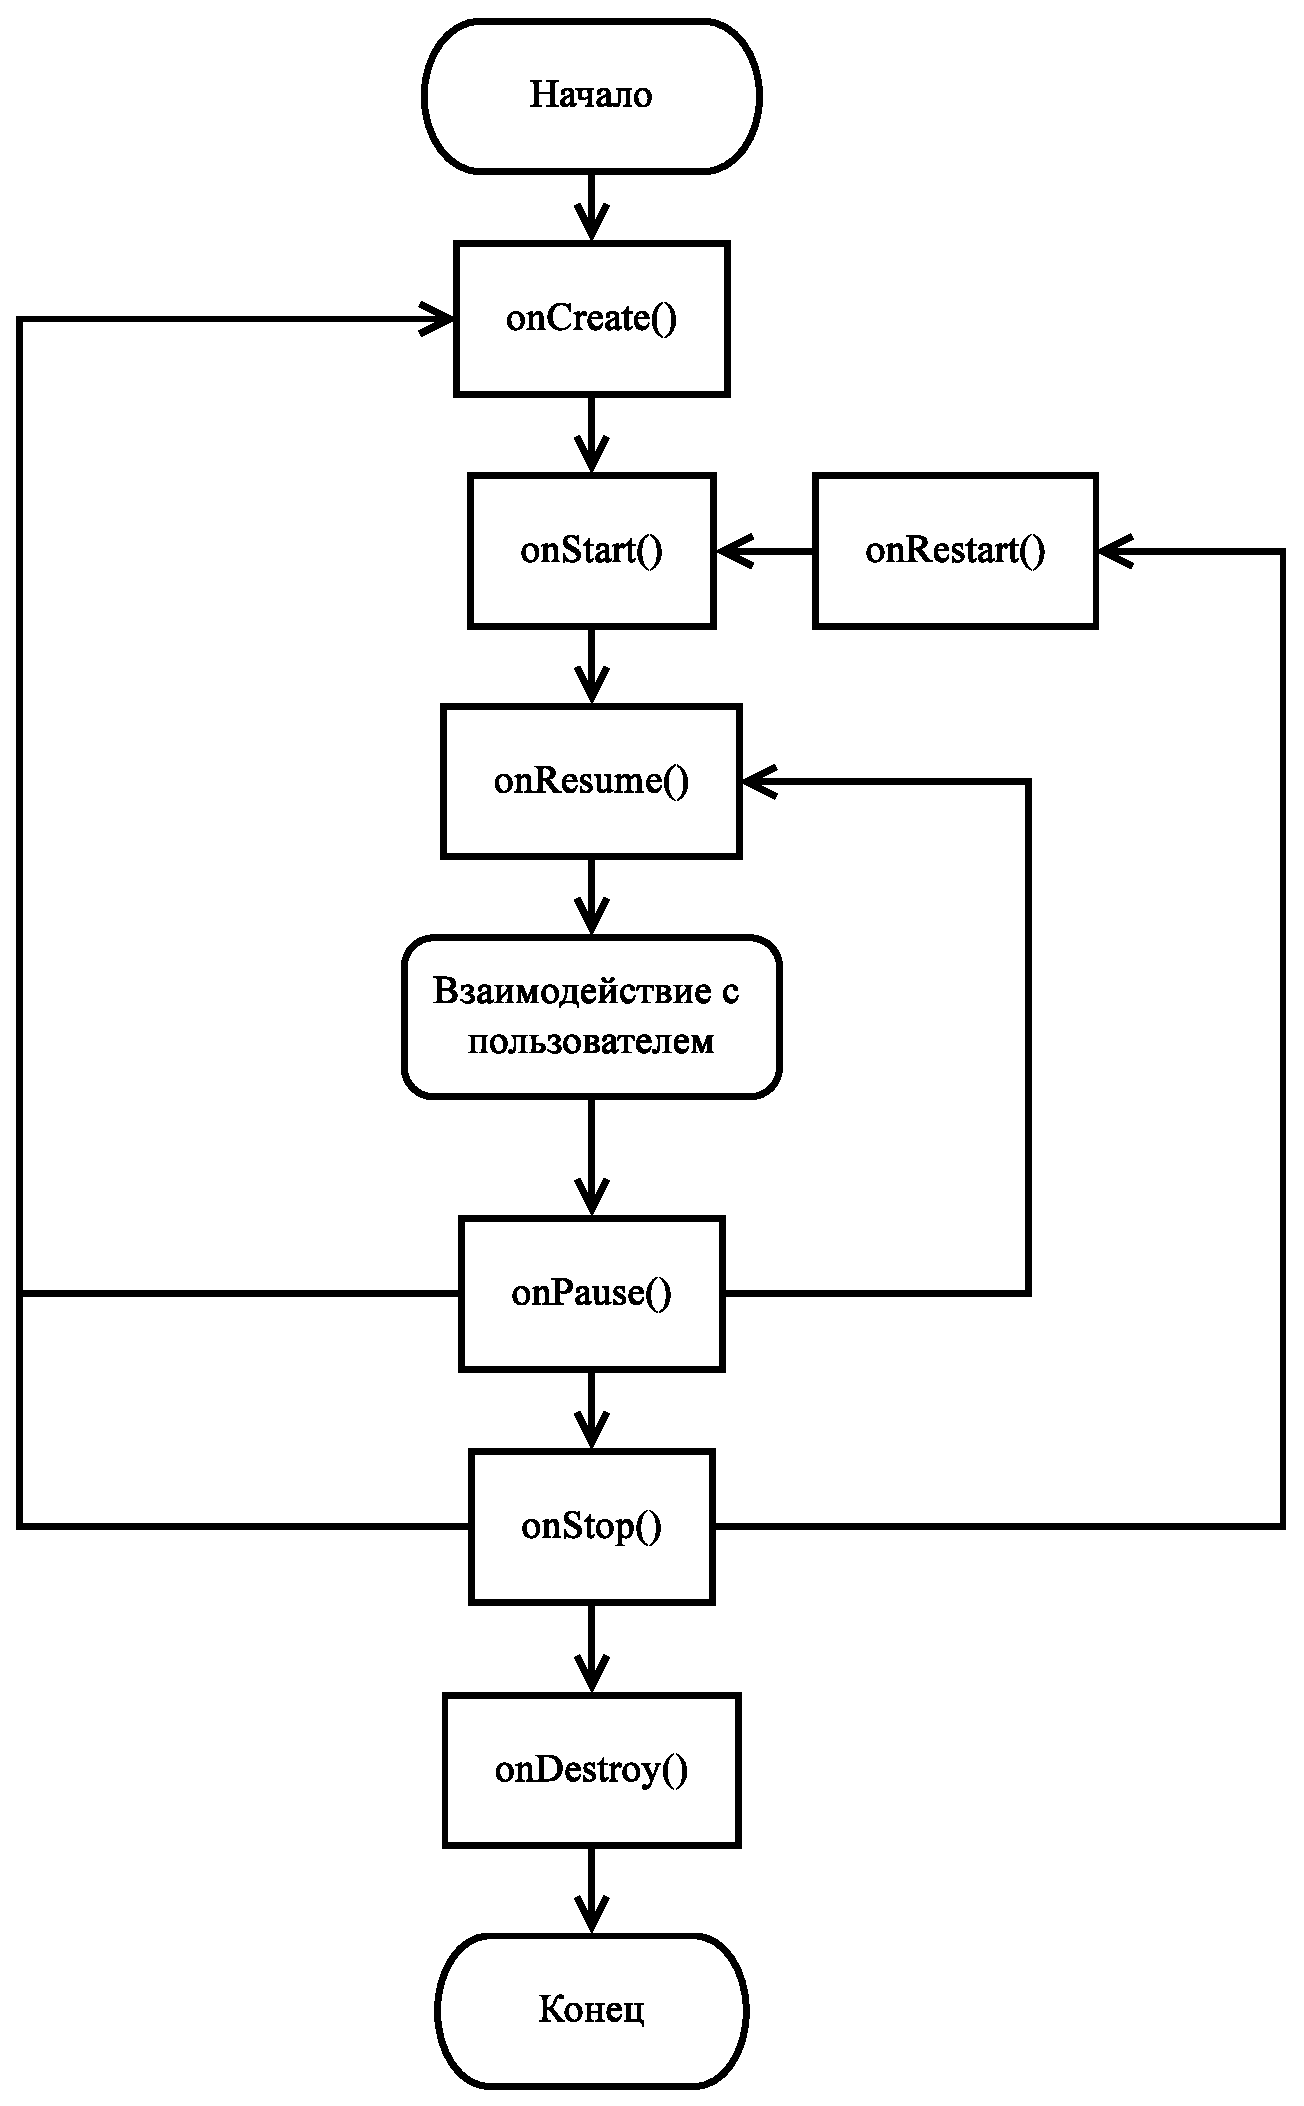
\includegraphics[width=110mm]{fig/implementation_ui_lifecycle_activity.eps}
  }
  \caption{Жизненный цикл экрана приложения}
  \label{fig:implementation_ui_lifecycle_activity}
\end{figure}

При создании экземпляра \textit{Activity} вызывается метод \textit{onCreate}.
Типичная реализация данного метода предполагает инициализацию
всех вложенных элементов интерфейса.
Далее вызываются методы \textit{onStart}, \textit{onResume},
и данный экран получает фокус.
При открытии различных вспдывающих окон у родительского экрана вызывается
метод \textit{onPause}, а при переходе на другой экран --- \textit{onStop}.
Пара методов \textit{onPause}/\textit{onResume} обычно используется для
сохранения/загрузки промежуточных результатов работы экрана.
Метод \textit{onDestroy} вызывается при закрытии приложения.
Данный метод часто переопределяется для освобождения используемых ресурсов.
Отметим, что жизненный цикл фрагмента имеет несколько более сложный вид
и связан с жизненным циклом родительского экрана.

Рассмотрим задачу организации форматирования и валидации данных.
Пользователь приложения должен иметь возможность ввода данных в
различные поля приложения.
Классы пользовательского приложения должны выполнять валидацию и форматирование
введенных данных и предоставлять их подсистеме обработки данных в совместимой форме.
Кроме этого, они должны поддерживать возможность автоматического
заполнения полей форматированными значениями в случае, если они заполнялись раньше.
Ситуация усложняется тем, что представление данных с точки зрения классов
пользовательского интерфейса Android и классов подсистемы обработки данных
приложения могут различаться.
Для решения данной задачи была разработан набор классов, представленный
на рисунке~\ref{fig:implementation_ui_edit_manager}.
В нем определяются интерфейсы параметризованные интерфейсы
\textit{IEditManager}, \textit{IFormatter}, \textit{IFormatter}
и набор их реализаций, связанных друг с другом. Рассмотрим каждый из них более подробно.
Интерфейс \textit{IFormatter} используется для форматирования некоторого входного
значения заданного типа, определенного шаблоном интерфейса.
Результатом работы единственного метода данного интерфейса является строка,
пригодная для размещения в элементе пользовательского интерфейса.
Метод \textit{validate} интерфейса \textit{IValidator} предназначен для
конвертации параметра-строки, соответствующей пользовательскому вводу,
в тип данных, совместимый с подсистемой обработки данных. В случае,
если подобная конвертация оказывается невозможной, он возбуждает
стандартное исключение типа \textit{IllegalArgumentException}.
Интерфейс \textit{IEditManager} определяет протокол взаимодействия
между фрагментом приложения, полем ввода данных
и подсистемой обработки данных.
Он имеет три метода, первые два из которых используются
для установки и получения последнего корректного введенного значения
в совместимом формате соответственно, а третий используется для проверки,
содержит ли поле ввода корректное значение в данный момент.

\begin{figure}[h!]
  \centering
  \fcolorbox{gray}{white}{
    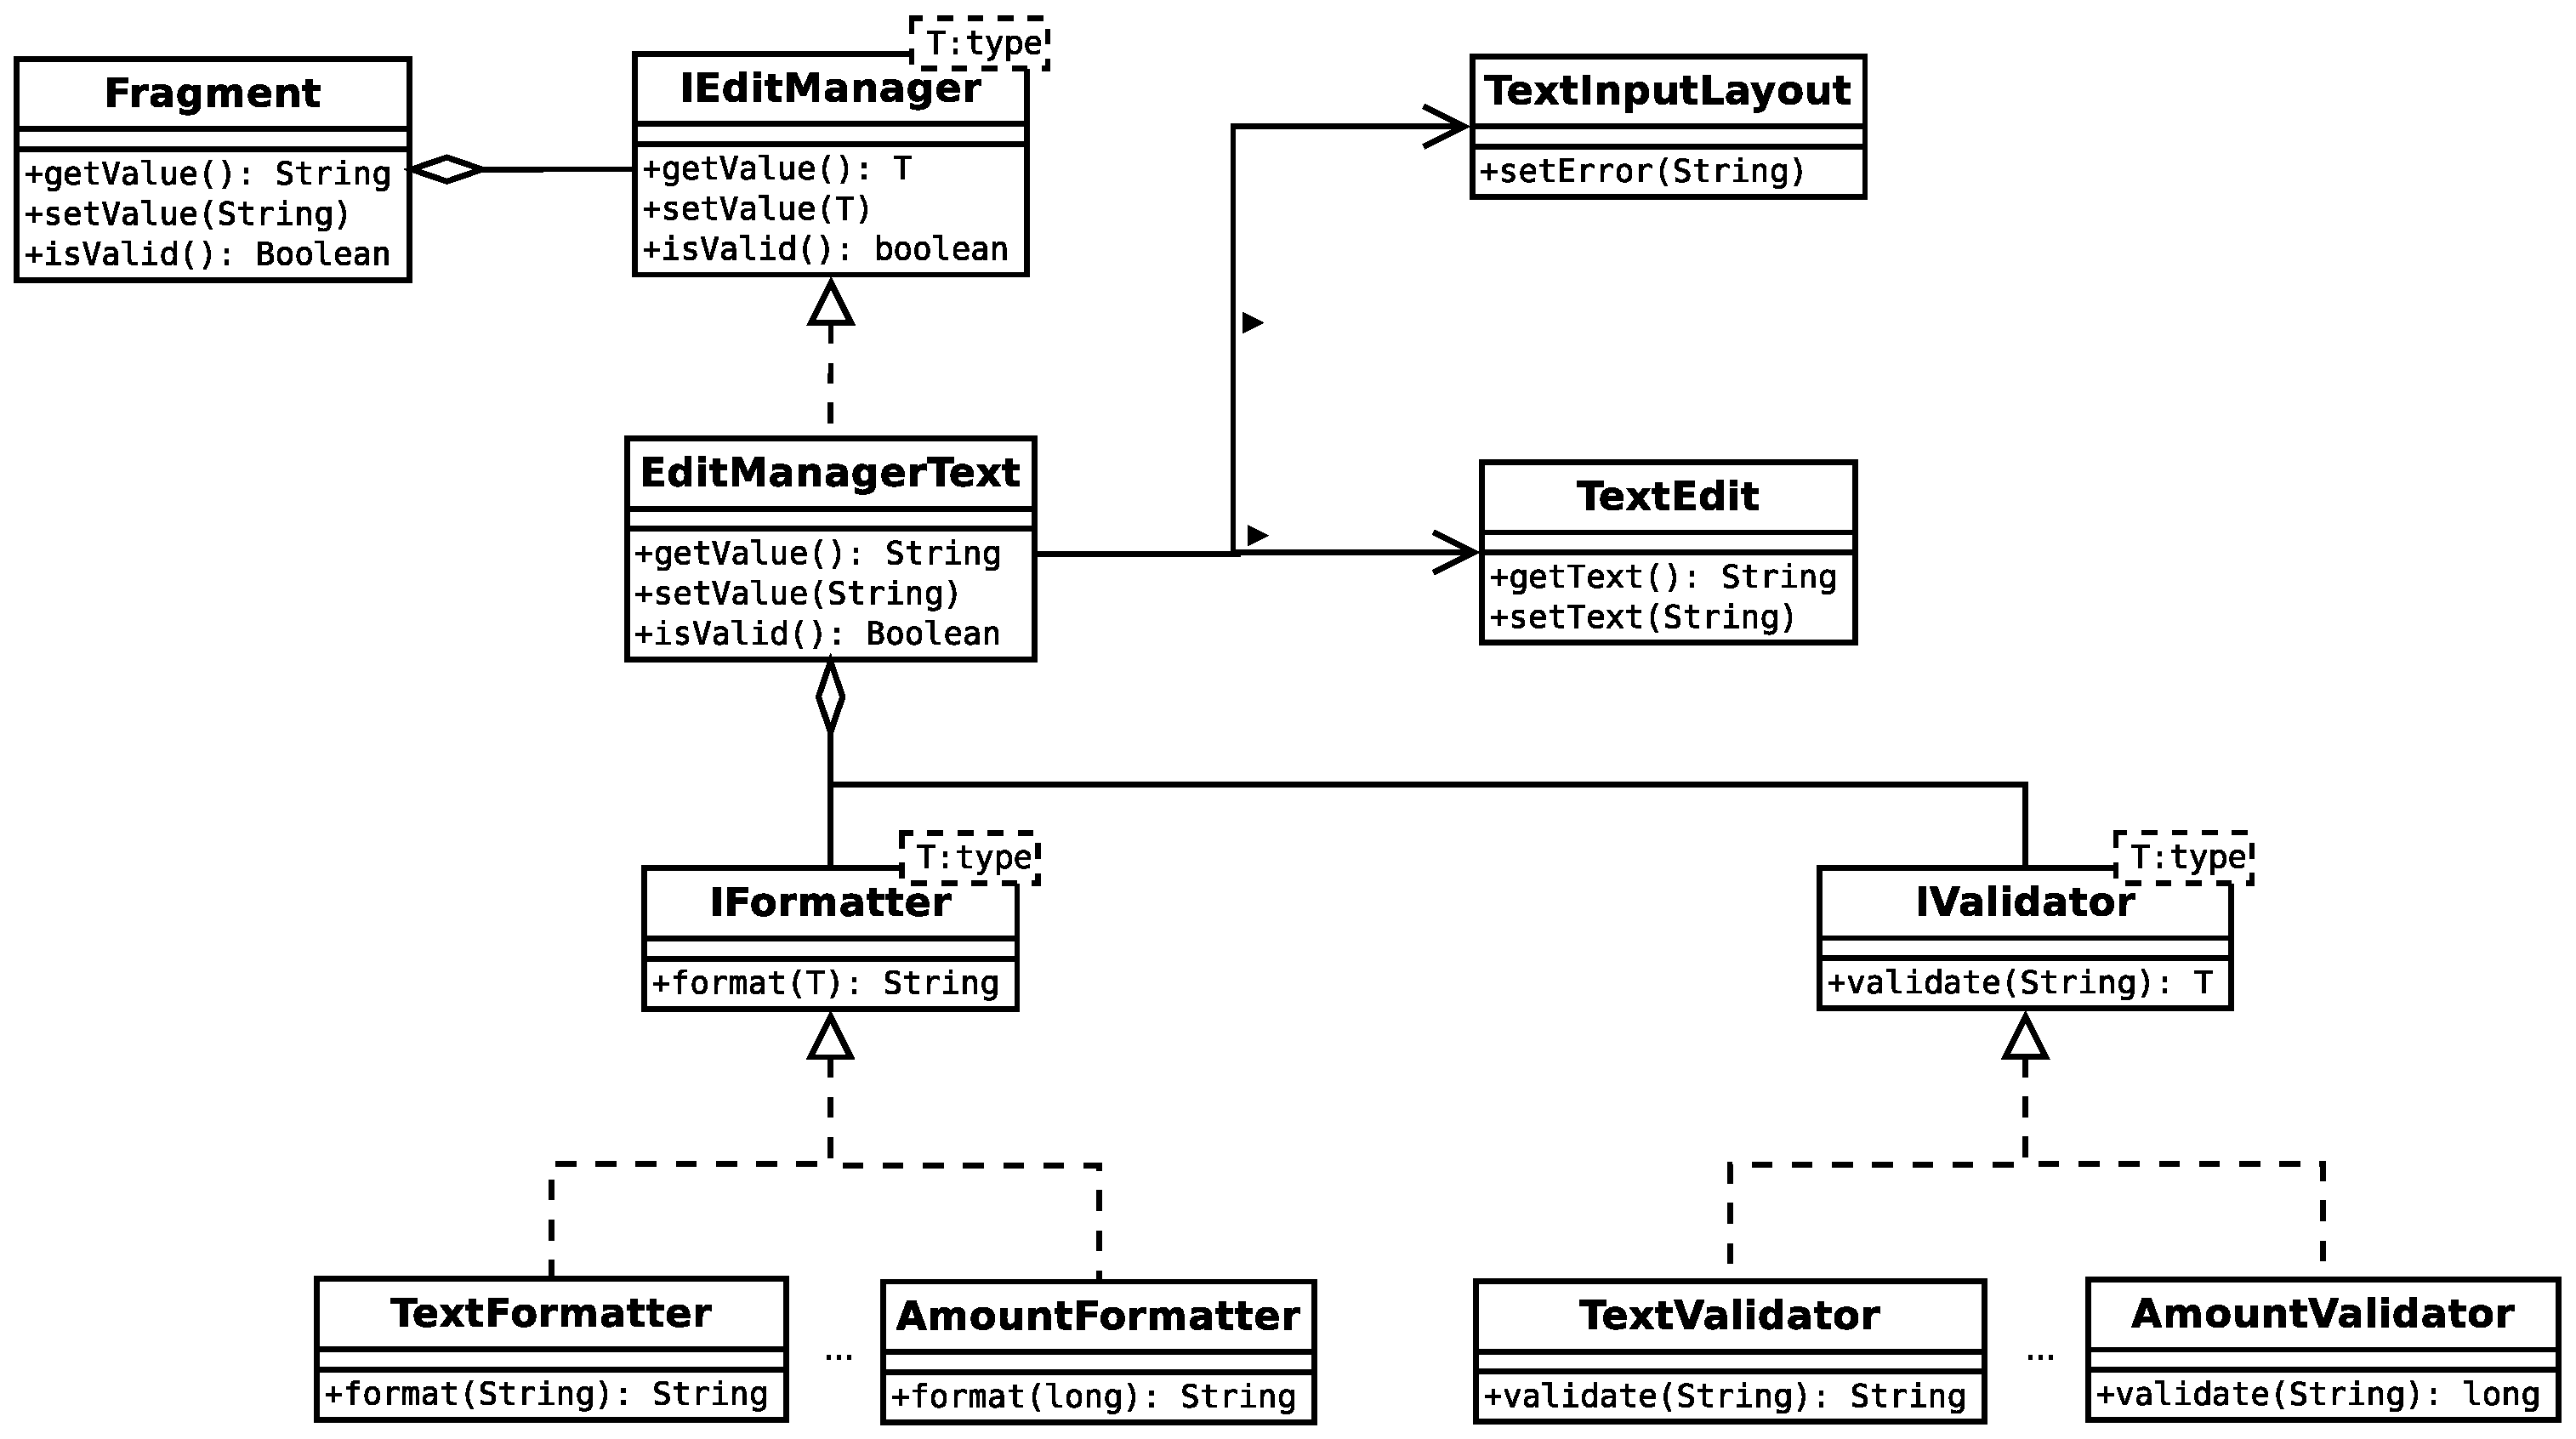
\includegraphics[width=140mm]{fig/implementation_ui_edit_manager.eps}
  }
  \caption{Диаграмма классов обработки данных, \\ вводимых пользователем}
  \label{fig:implementation_ui_edit_manager}
\end{figure}

Взаимодействие описанных сущностей осуществляется следующим образом.
Экран или фрагмент в ходе своего жизненного цикла создают экземпляр класса,
реализующего интерфейс \textit{IEditManager}, и связывает его с целевыми
полями ввода и прочими вспомогательными объектами.
Конкретная реализация интерфейса \textit{IEditManager}
(например, \textit{EditManagerText})
создает необходимые ей экземлпяры классов, реализующих интерфейсы
\textit{IFormatter} (\textit{TextFormatter})
и \textit{IValidator} (\textit{TextValidator}),
и использует их в своей реализации,
подставляя результаты вызова методов объекто этих классов
в качестве собственных выходных значений.

Отметим, что разработанный набор классов получился весьма гибким.
Он используется для обработки и отображения всех вводимых в приложение данных.
Кроме этого, для отображения данных в полях, не допускащих редактирования,
вместо интерфейса \textit{IEditManager} используется подобный ему \textit{IViewManager}.
Данный интерфейс отличается тем, что в нем предусмотрена возможность чтения данных.
В связи с этим у реализующих его классов отсутствует необходимость
использования функциональности, предоставляемой реализациями интерфейса \textit{IValidator}.

Рассмотрим пользовательский интерфейс основных экранов приложения.
На рисунке~\ref{fig:implementation_ui_activity_balance_text}
представлен главный экран приложения в
текстовом режиме представления данных.

\begin{figure}[h!]
  \centering
  \fcolorbox{gray}{white}{
    \includegraphics[width=140mm]{fig/implementation_ui_activity_balance_text.eps}
  }
  \caption{Главный экран (текстовый режим)}
  \label{fig:implementation_ui_activity_balance_text}
\end{figure}

Данный экран предназначен для отображения текущей финансовой
информации пользователя. Основными его элементами являются:
\begin{itemize}
\item виджет выбора промежутка учета;
\item виджет выбора учетной записи;
\item поле суммы денежных средств текущей учетной записи;
\item список связанных изменений баланса;
\item кнопка добавления изменения баланса.
\end{itemize}

По умолчанию элементы списка содержат величину изменения баланса,
список связанных категорий, а также дату регистрации изменения.
С помощью переключателя, расположенного во вспомогательном меню,
пользователь может включить группировку данных.
В этом случае список изменений баланса содержит сведения
об изменениях баланса за выбранный период,
сгрупированные по категориям учета.
С помощью кнопок, расположенных в верхней части экрана, пользователь
может открыть главное меню приложения или вспомогательное меню экрана.
При нажатии на любой элемент списка пользователь переходит
на экран редактирования изменения баланса,
при этом поля нового экрана заполняются автоматически.
С помощью переключателя, расположенного во вспомогательном меню,
пользователь может перейти в графический режим, представленный
на рисунке~\ref{fig:implementation_ui_activity_balance_graphic}.

\begin{figure}[h!]
  \centering
  \fcolorbox{gray}{white}{
    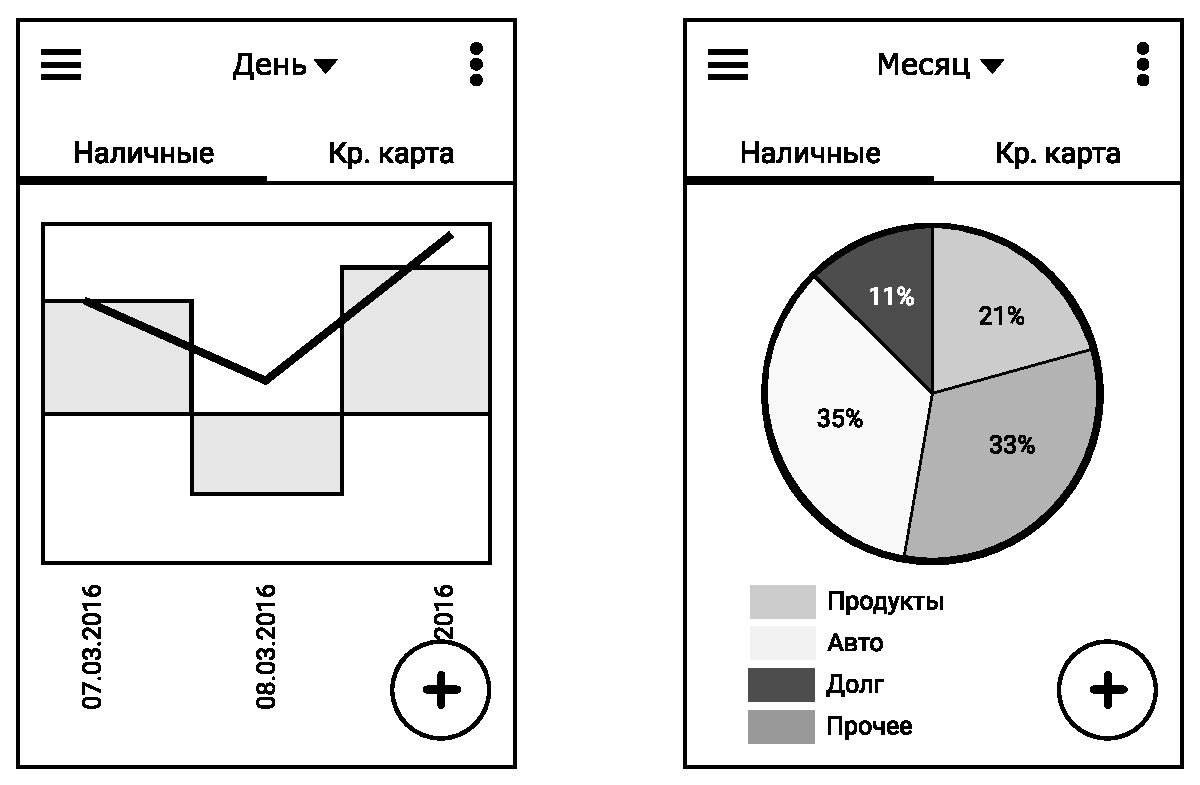
\includegraphics[width=140mm]{fig/implementation_ui_activity_balance_graphic.eps}
  }
  \caption{Главный экран (графический режим)}
  \label{fig:implementation_ui_activity_balance_graphic}
\end{figure}

Содержание и поведение данного экрана в графическом режиме также
определяется состоянием переключателя группировки данных.
Если группировка данных выключена,
пользователю показывается график изменения баланса учетной записи.
На оси ординат данного графика расположены значения,
соответствующие величинам изменений баланса, а на оси абсцисс ---
даты в соответствии с выбранным масштабом промежутков учета.
На графике расположены как абсолютные значения изменений баланса,
сгруппированные по промежуткам учета (показаны в виде столбцов),
так и изменение значения суммы денежных средств на счете
на конечный момент каждого промежутка учета (показано в виде ломаной).
Выбор размера промежутка учета осуществляется с помощью виджета,
расположенного в верхней части экрана.
Если группировка данных включена, пользователю показывается
круговая диаграмма, представляющая распределение изменений баланса
по категориям за промежуток учета, также выбирамый с помощью виджета,
расположенного в верхней части экрана.
Следует отметить, что изменения баланса, связанные с несколькими
категориями учета, учитываются в сегменте каждой категории отдельно,
поэтому наибольший вклад в размер сегмента будут вносить изменения
баланса, связанные с одной категорией учета.
При нажатии на кнопку добавления изменения баланса,
расположенную в правом нижнем углу,
пользователь переходит на экран редактирования изменений баланса,
представленный на рисунке~\ref{fig:implementation_ui_activity_input}.

\begin{figure}[h!]
  \centering
  \fcolorbox{gray}{white}{
    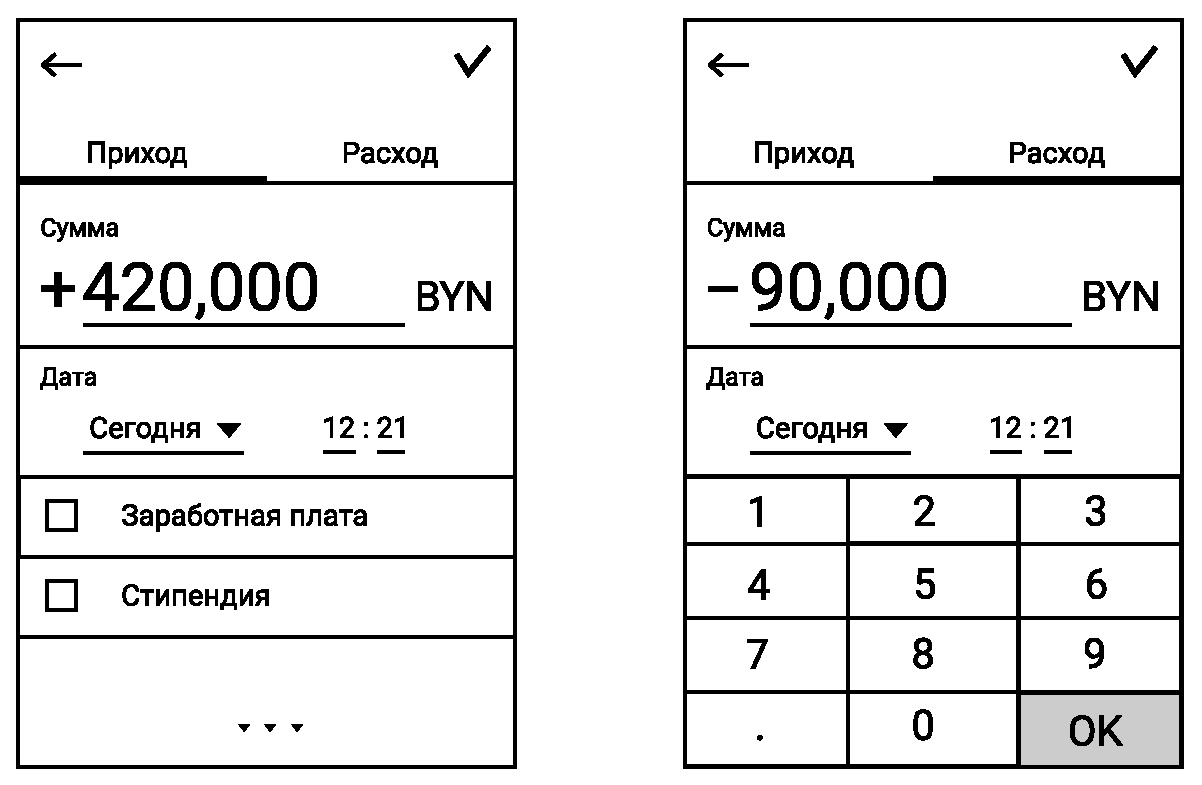
\includegraphics[width=140mm]{fig/implementation_ui_activity_input.eps}
  }
  \caption{Экран редактирования изменений баланса}
  \label{fig:implementation_ui_activity_input}
\end{figure}

Данный экран содержит следующие элементы интерфейса:
\begin{itemize}
\item переключатель типа изменения баланса (расход/приход);
\item поле ввода величины изменения баланса;
\item поле ввода даты учета;
\item список категорий учета.
\end{itemize}

Содержимое списка категорий учета зависит от типа редактируемого
изменения баланса, при этом с каждом изменением баланса можно связать несколько
категорий учета.
При вводе величины изменения баланса пользователю показывается цифровая клавиатура.
Следует отметить, что при добавлении изменения баланса поле редактирования
даты учета пользователю не показывается, а сама дата устанавливается автоматически.
Это сделано для того, чтобы мотивировать пользователей
вводить свои финансовые данные как можно быстрее,
желатьельно сразу после осуществления фактических транзакций.
С помощью кнопок, расположенных в верхней части экрана, пользователь
может сохранить изменения или вернуться на предыдущий экран.

С помощью главного меню приложения пользователь может перейти на
экран просмотра учетных записей, содержащий список всех учетных записей,
и связанный с ним экран редактирования выбранной учетной записи.
Данные экраны представлены на рисунке~\ref{fig:implementation_ui_activity_account}.

\begin{figure}[h!]
  \centering
  \fcolorbox{gray}{white}{
    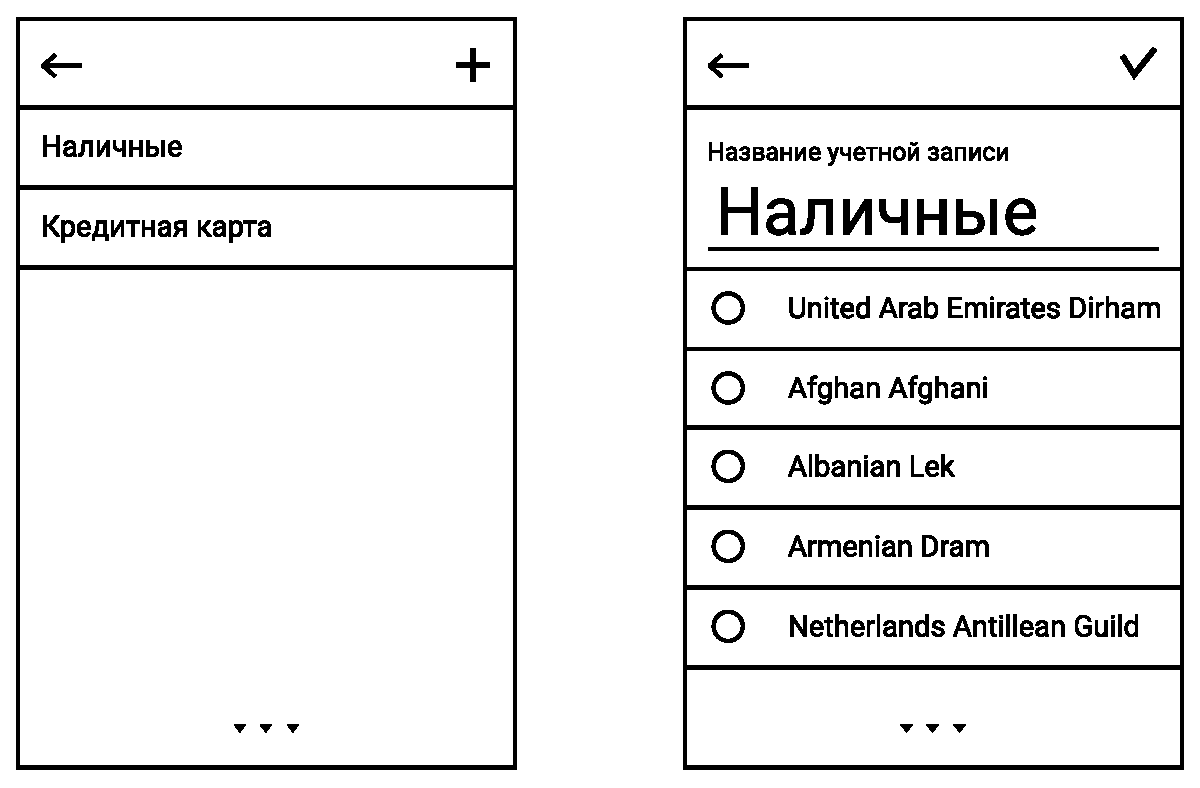
\includegraphics[width=140mm]{fig/implementation_ui_activity_account.eps}
  }
  \caption{Экраны управления учетными записями}
  \label{fig:implementation_ui_activity_account}
\end{figure}

Экран просмотра позволяет выполнять основные операции
со списком учетных записей.
Создание новых записей производится путем нажатия на кнопку,
расположенную в верхнем правом углу экрана просмотра списка записей.
Удаление записи производится путем сдвига соответствующего элемента списка;
редактирование --- путем нажатия на него.
Создание и редактирование учетных записей производится с помощью
отдельного экрана.
Кроме этого, пользователь имеет возможность выбора порядка следования
учетных записей. Для изменения порядка записи в списке требуется
выполнить долгое нажатие на данную запись и перетащить ее в требуемое место.

Экран редактирования позволяет добавить новую или изменить выбранную
учетную запись. Данный экран состоит из поля ввода названия учетной записи,
а также списка валют учета, из которого пользователю требуется выбрать необходимую.
С помощью кнопок, расположенных в верхней части экрана, пользователь
может сохранить изменения или вернуться на предыдущий экран.

С помощью главного меню приложения пользователь может перейти на
экран просмотра категорий учета, содержащий список всех категорий учета,
и связанный с ним экран редактирования выбранной категории учета.
Данные экраны представлены на рисунке~\ref{fig:implementation_ui_activity_category}.

\begin{figure}[h!]
  \centering
  \fcolorbox{gray}{white}{
    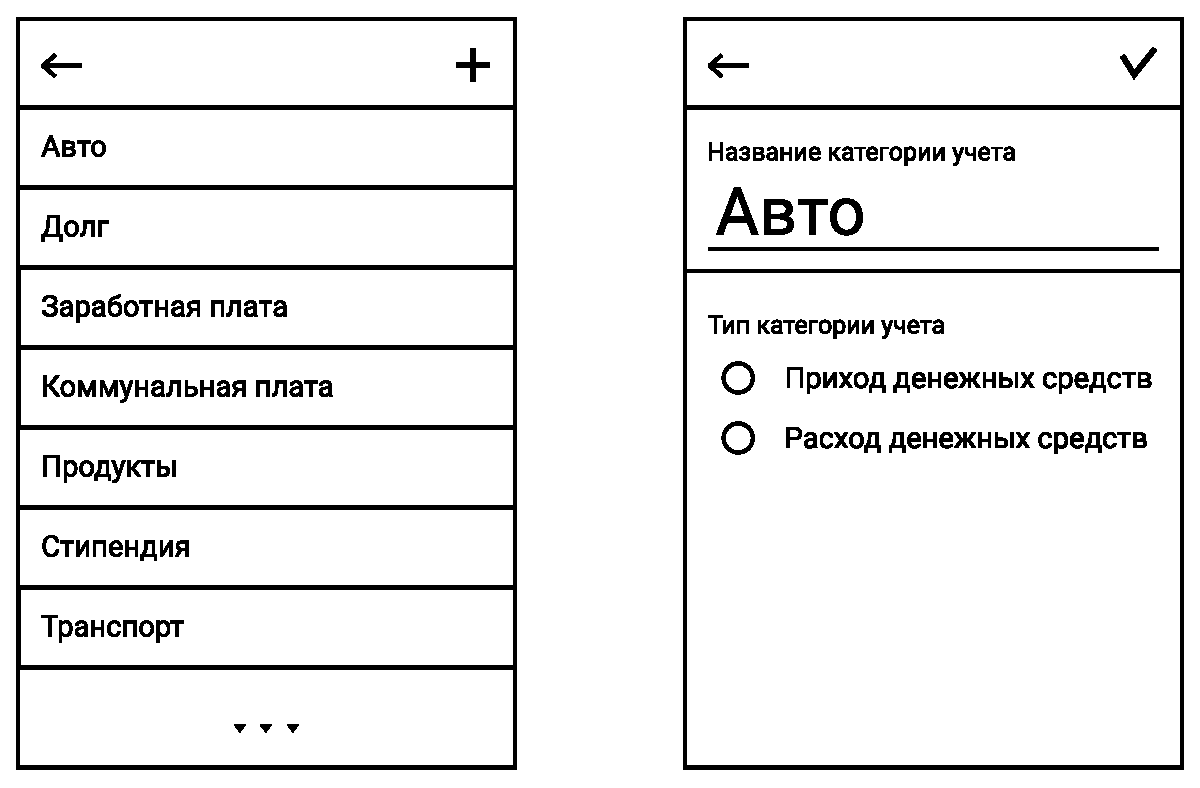
\includegraphics[width=140mm]{fig/implementation_ui_activity_category.eps}
  }
  \caption{Экраны управления категориями учета}
  \label{fig:implementation_ui_activity_category}
\end{figure}

Экран просмотра позволяет выполнять основные операции
со списком категорий ввода.
Создание новых категорий производится путем нажатия на кнопку,
расположенную в верхнем правом углу экрана просмотра списка записей.
Удаление записи производится путем сдвига соответствующего элемента списка;
редактирование --- путем нажатия на него.
Создание и редактирование категорий учета производится также
с помощью отдельного экрана.

Экран редактирования позволяет добавить новую или изменить выбранную
учетную запись. Данный экран состоит из поля ввода названия категории учета,
а также переключателя выбора типа категории (приход/расход).
С помощью кнопок, расположенных в верхней части экрана, пользователь
может сохранить изменения или вернуться на предыдущий экран.

Приложение имеет и некоторые другие экраны, например,
экран настроек или экран распознавания изображений.
Поскольку множество возлагаемых на них функций
и пользовательский интерфейс данных экранов является объектом для
изменений, в данном разделе они не рассматриваются.


\subsection{Реализация подсистемы обработки данных}
\label{subsec:implementation_bl}

Подсистема обработки данных представляет собой связующее звено
между подсистемами хранения данных, компьютерного зрения и
пользовательским интерфейсом, играя ключевую роль в работе всего приложения.
Поскольку данная подсистема соответствует блоку Presenter шаблона
MVP, ее реализация состоит из набора классов и интерфейсов,
имеющих в составе своего названия данное ключевое слово.
На рисунке~\ref{fig:implementation_bl_presenter} представлена схема взаимодействия
классов графического интерфейса и классов подсистемы обработки данных.

\begin{figure}[h!]
  \centering
  \fcolorbox{gray}{white}{
    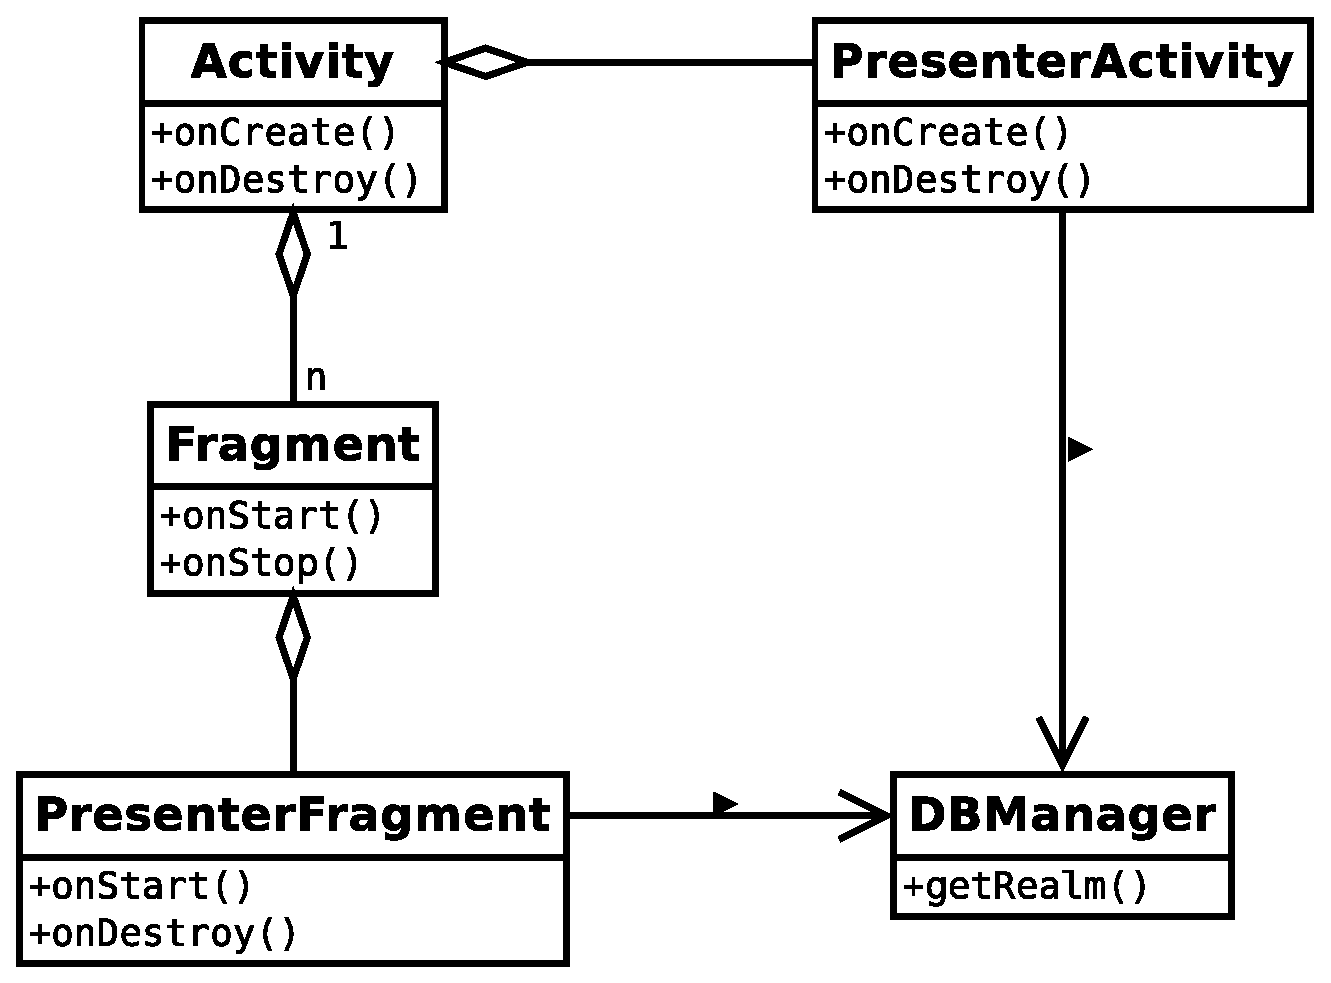
\includegraphics[width=140mm]{fig/implementation_bl_presenter.eps}
  }
  \caption{Схема использования классов \\ подсистемы обработки данных}
  \label{fig:implementation_bl_presenter}
\end{figure}

Классы \textit{Activity} и \textit{Fragment} в ходе своего жизненного цикла
создают объекты классов \textit{PresenterActivity} и \textit{PresenterFragment}.
Интерфейсы классов \textit{Presenter*} имеют следующие особенности:
\begin{itemize}
  \item привязаны к жизненному циклу родительских объектов;
  \item принимают в качестве аргументов объекты типа \textit{Bundle};
  \item инкапсулируют набор рабочих данных и объекты Realm.
\end{itemize}

Данные объекты также инкапсулируют все необходимые алгоритмы обработки данных и
имеют доступ к подсистеме хранения данных приложения (класс \textit{DBManager}).
Объекты классов графического интерфейса перенаправляют
им свои запросы загрузки, обработки и хранения данных,
используя индексы требуемых им объектов в списках хранения данных.

Подводя итог рассмотрению реализации частей приложения, отметим,
что в целом их структура разработана таким образом,
чтобы избегать циклов в графе взаимодействия их объектов.
Данная особенность позволила существенно упростить
структуру проекта в целом и его подсистем в частности.

\subsection{Тестирование программного модуля}

Существует как минимум три основных метода тестирования
программного обеспечения:
\begin{itemize}
\item ручное;
\item автоматизированное;
\item модульное.
\end{itemize}

Ручное тестирование представляет собой активное использование приложения
с целью выявления ошибок в его работе.
Автоматизированное тестирование отличается от ручного тем,
что в его случае сам алгоритм использования приложения также запрограммирован.
Данный вид тестирования, называемый также регрессионным,
позволяет сравнительно быстро определить,
внесли ли новые изменения в код приложения новые ошибки в ход его работы.
Модульное тестирование используется по сути с той же целью,
что и автоматизированное. Основные отличия заключаются в том,
что модульные тесты пишутся разработчиками приложения,
тестируют части кода приложения, а не все приложение в целом
и имеют значительно меньшие размер и время выполнения.

Существует определенная специфика в механизме тестирования приложений
для платформы Android. Суть её сводится к разделению множества модульных тестов
на тесты, выполняемые на компьютере разработчика, и на инструментальные тесты,
выполняемые на целевом устройстве.
Основной причиной подобного разделения является необходимость тестирования
графического интерфейса приложения, а также существование ошибок,
проявляющихся лишь на определенных версиях мобильной платформы.
С другой стороны, многие модульные тесты не зависят от
целевой платформы (вследствие кроссплатформенности виртуальной машины Java)
и могут выполняться значительно быстрее на компьютере разработчика.

В рамках реализации данного проекта были разработан набор модульных тестов,
покрывающих ключевую функциональность приложения.
Использование паттерна проектирования MVP позволило существенно упростить их написание.
Дело в том, что одной из особенностей данного паттерна является возможность
определения интерфейсов \textit{IPresenter*} и использования
их в классах-клиентах вместо конкретных реализаций \textit{Presenter*},
как показано на рисунке~\ref{fig:implementation_testing_presenter}.

\begin{figure}[h!]
  \centering
  \fcolorbox{gray}{white}{
    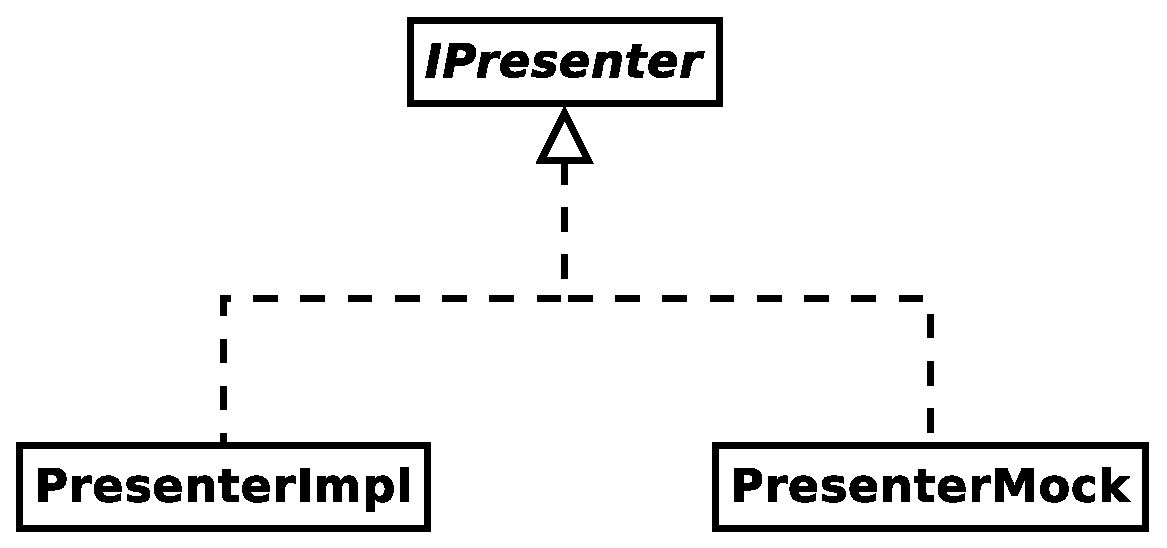
\includegraphics[width=82mm]{fig/implementation_testing_presenter.eps}
  }
  \caption{Схема эмуляции классов \\ подсистемы обработки данных}
  \label{fig:implementation_testing_presenter}
\end{figure}

Данный подход позволяет
отделить интерфейс классов подсистемы обработки данных от реализации
для использования классов-заглушек (\textit{PresenterMock*}).
Классы-заглушки удобно использовать для тестирования классов подсистем-клиентов.
В начале каждого теста производится создание объекта тестируемого класса,
сопровождающегося подменой используемого им \textit{Presenter*}
на \textit{PresenterMock*}.
Методы объектов классов-заглушек вместо действий, предписанных их контрактами,
выполняют действия, направленные на облегчение тестирования классов-клиентов.

\subsection{Руководство пользователя}

Для использования приложения требуется скачать исходный код
приложения с публично доступного ресурса~\cite{github_money_keeper},
выполнить его компиляцию и установку.
Выполним описание базовых сценариев использования приложения.
Будем отмечать пронумерованными маркерами последовательность действий,
необходимых для выполнения каждого описываемого сценария.

Для того, чтобы добавить новую учетную запись, необходимо выполнить
последовательность действий, представленную на
рисунке~\ref{fig:implementation_manual_account}:
\begin{enumerate}
  \item Открыть главное меню путем нажатия на кнопку,
    расположенную в верхнем левом углу экрана приложения.
  \item
    Выбрать пункт <<Учетные записи>>.
  \item В появившемся экране просмотра учетных записей
    нажать на кнопку, расположенную в верхнем правом углу.
  \item В появившемся экране добавления/редактирования
    учетных записей указать название, а также используемую валюту ввода.
    Сохранить изменения путем нажатия на кнопку, расположенную
    в верхнем правом углу.
\end{enumerate}

\begin{figure}[h!]
  \centering
  \fcolorbox{gray}{white}{
    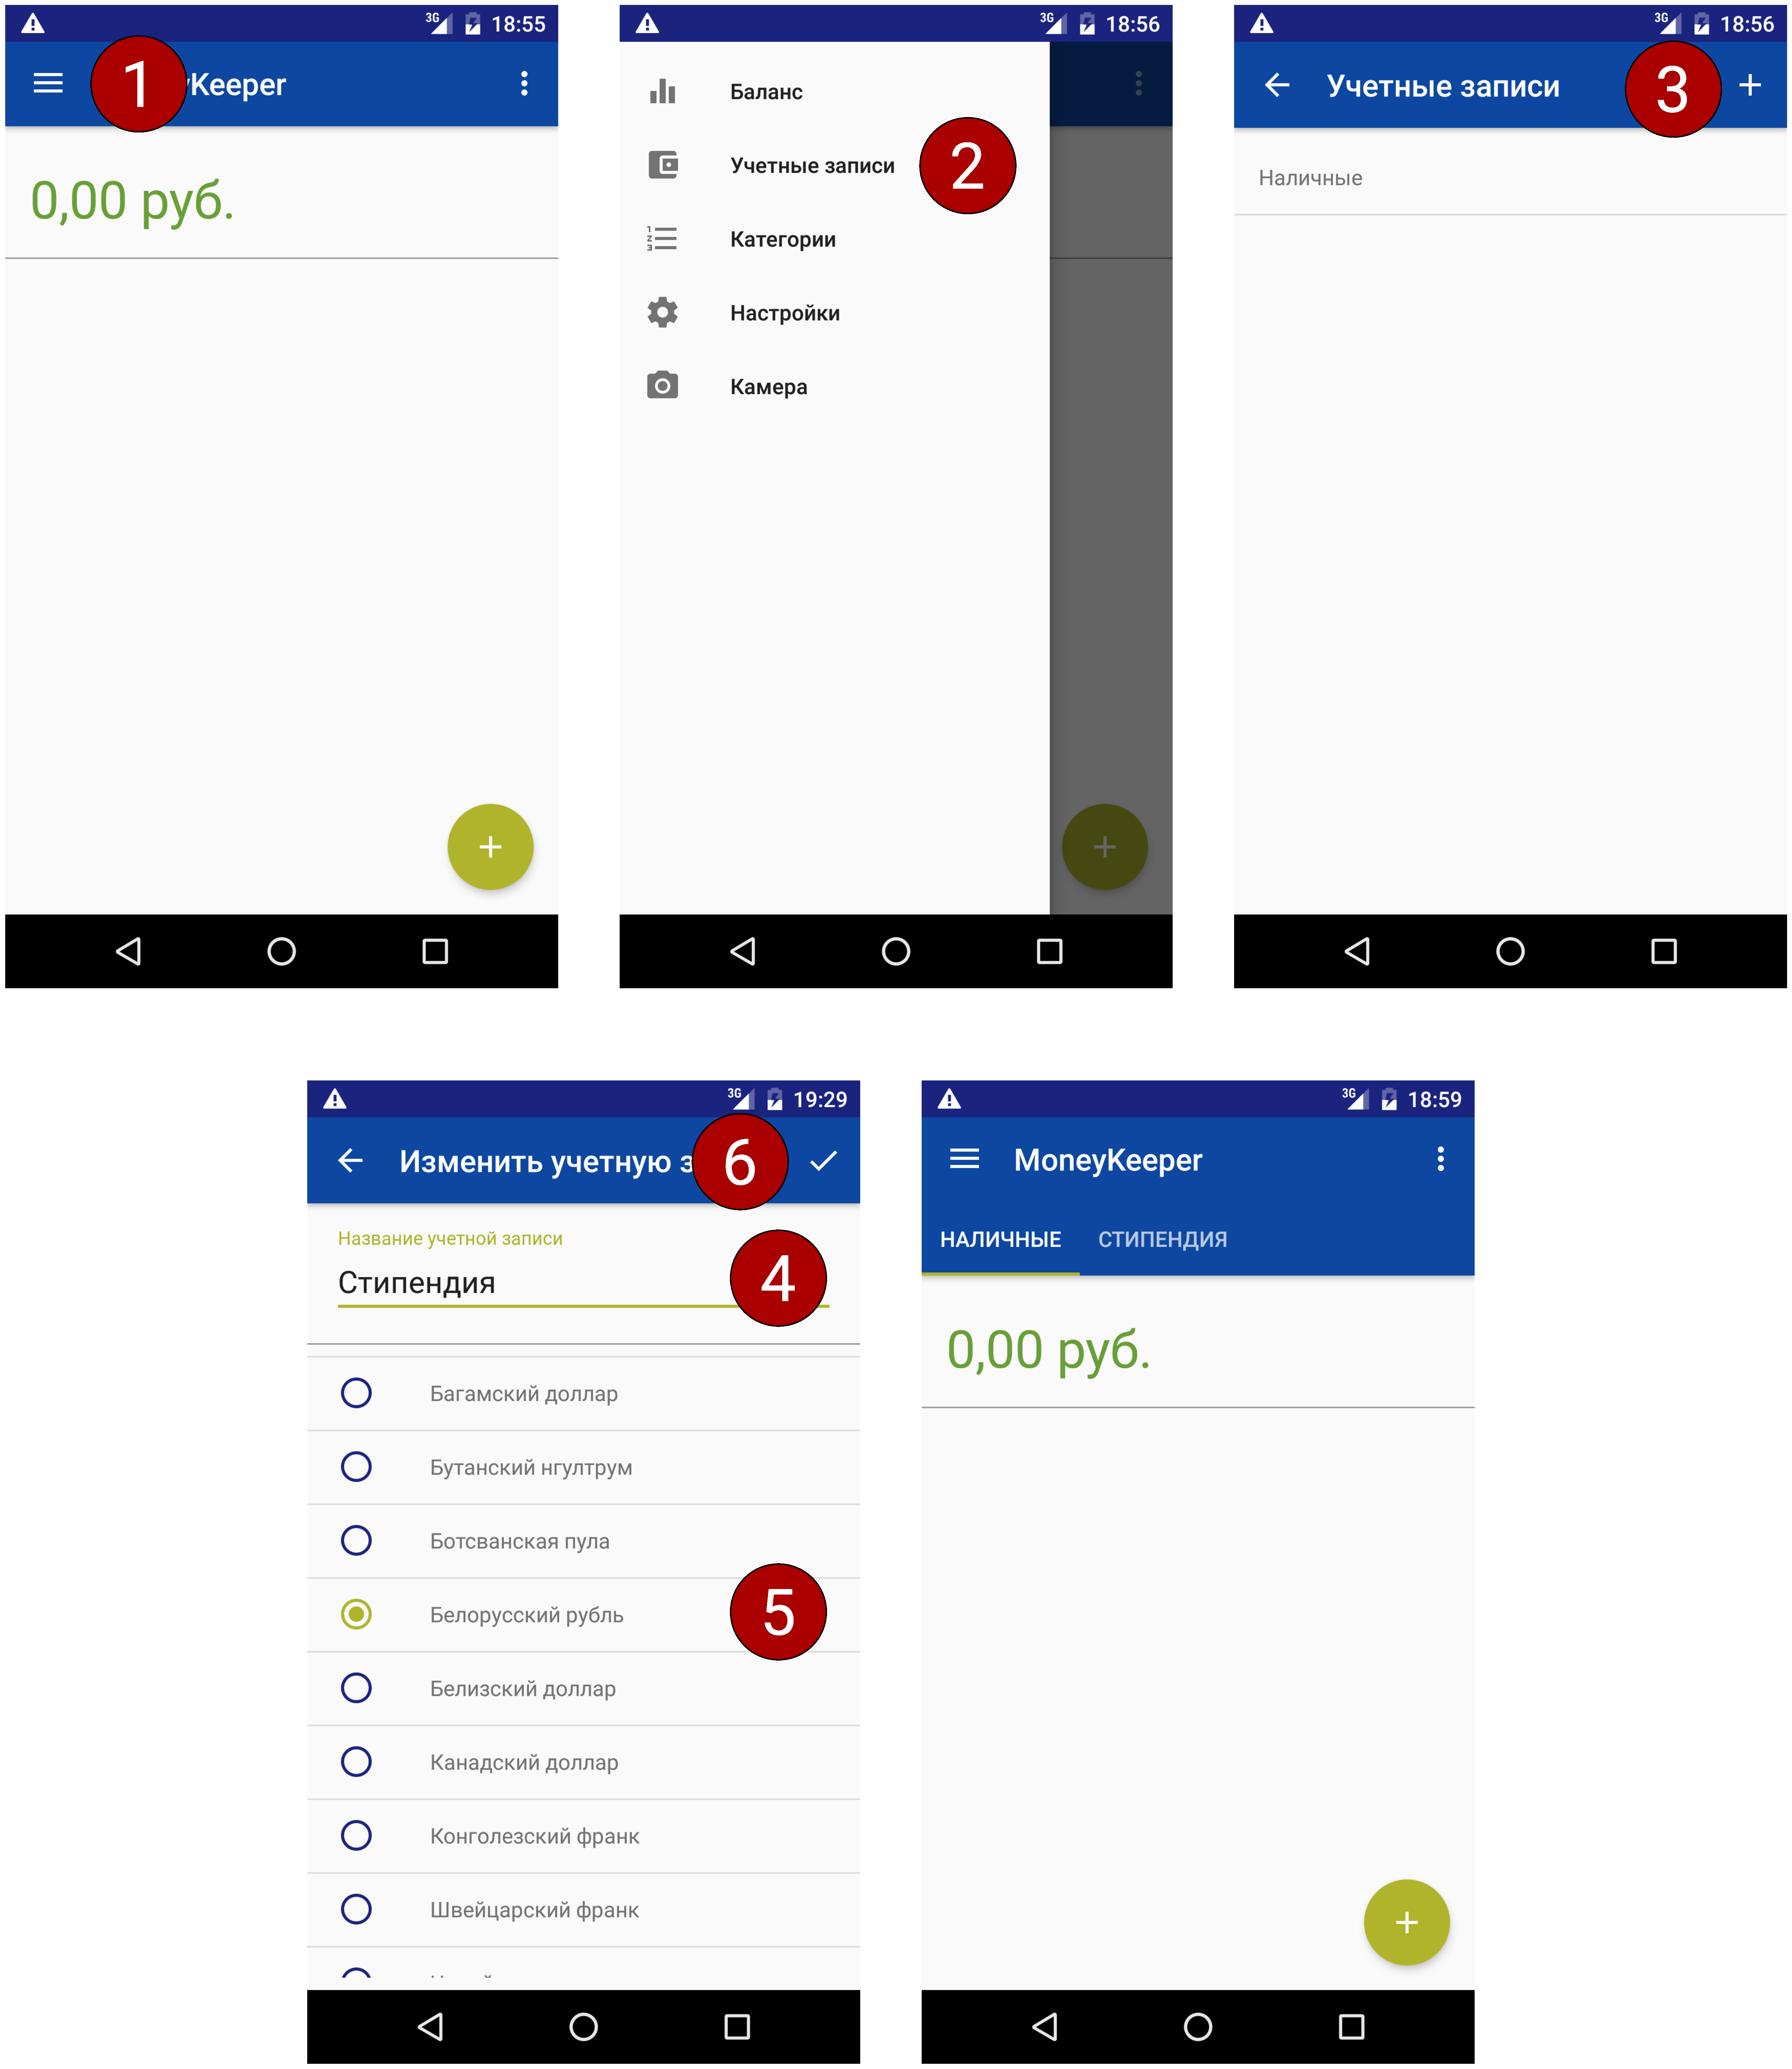
\includegraphics[width=140mm]{fig/implementation_manual_account.eps}
  }
  \caption{Добавление учетной записи}
  \label{fig:implementation_manual_account}
\end{figure}

Для того, чтобы добавить новую категорию учета, необходимо выполнить
последовательность действий, представленную на
рисунке~\ref{fig:implementation_manual_category}:
\begin{enumerate}
  \item Открыть главное меню.
  \item Выбрать пункт <<Категории>>.
  \item В появившемся экране просмотра категорий учета
    нажать на кнопку, расположенную в верхнем правом углу.
  \item В появившемся экране добавления/редактирования
    категорий учета указать название, а также тип категории.
    Сохранить изменения.
\end{enumerate}

\begin{figure}[h!]
  \centering
  \fcolorbox{gray}{white}{
    
\includegraphics[width=140mm]{fig/implementation_manual_category.eps}
  }
  \caption{Добавление категории учета}
  \label{fig:implementation_manual_category}
\end{figure}

Для того, чтобы добавить новое изменение баланса, необходимо выполнить
последовательность действий, представленную на
рисунке~\ref{fig:implementation_manual_balance_change}:
\begin{enumerate}
  \item Находясь на экране просмотра баланса, нажать на кнопку,
    раположенную в нижнем правом углу.
  \item В появившемся экране добавления/редактирования
    изменений баланса выбрать тип изменения (приход/расход) путем сдвига экрана.
    Указать величину изменения баланса и связанные категории.
    Сохранить изменения.
\end{enumerate}

\begin{figure}[h!]
  \centering
  \fcolorbox{gray}{white}{
    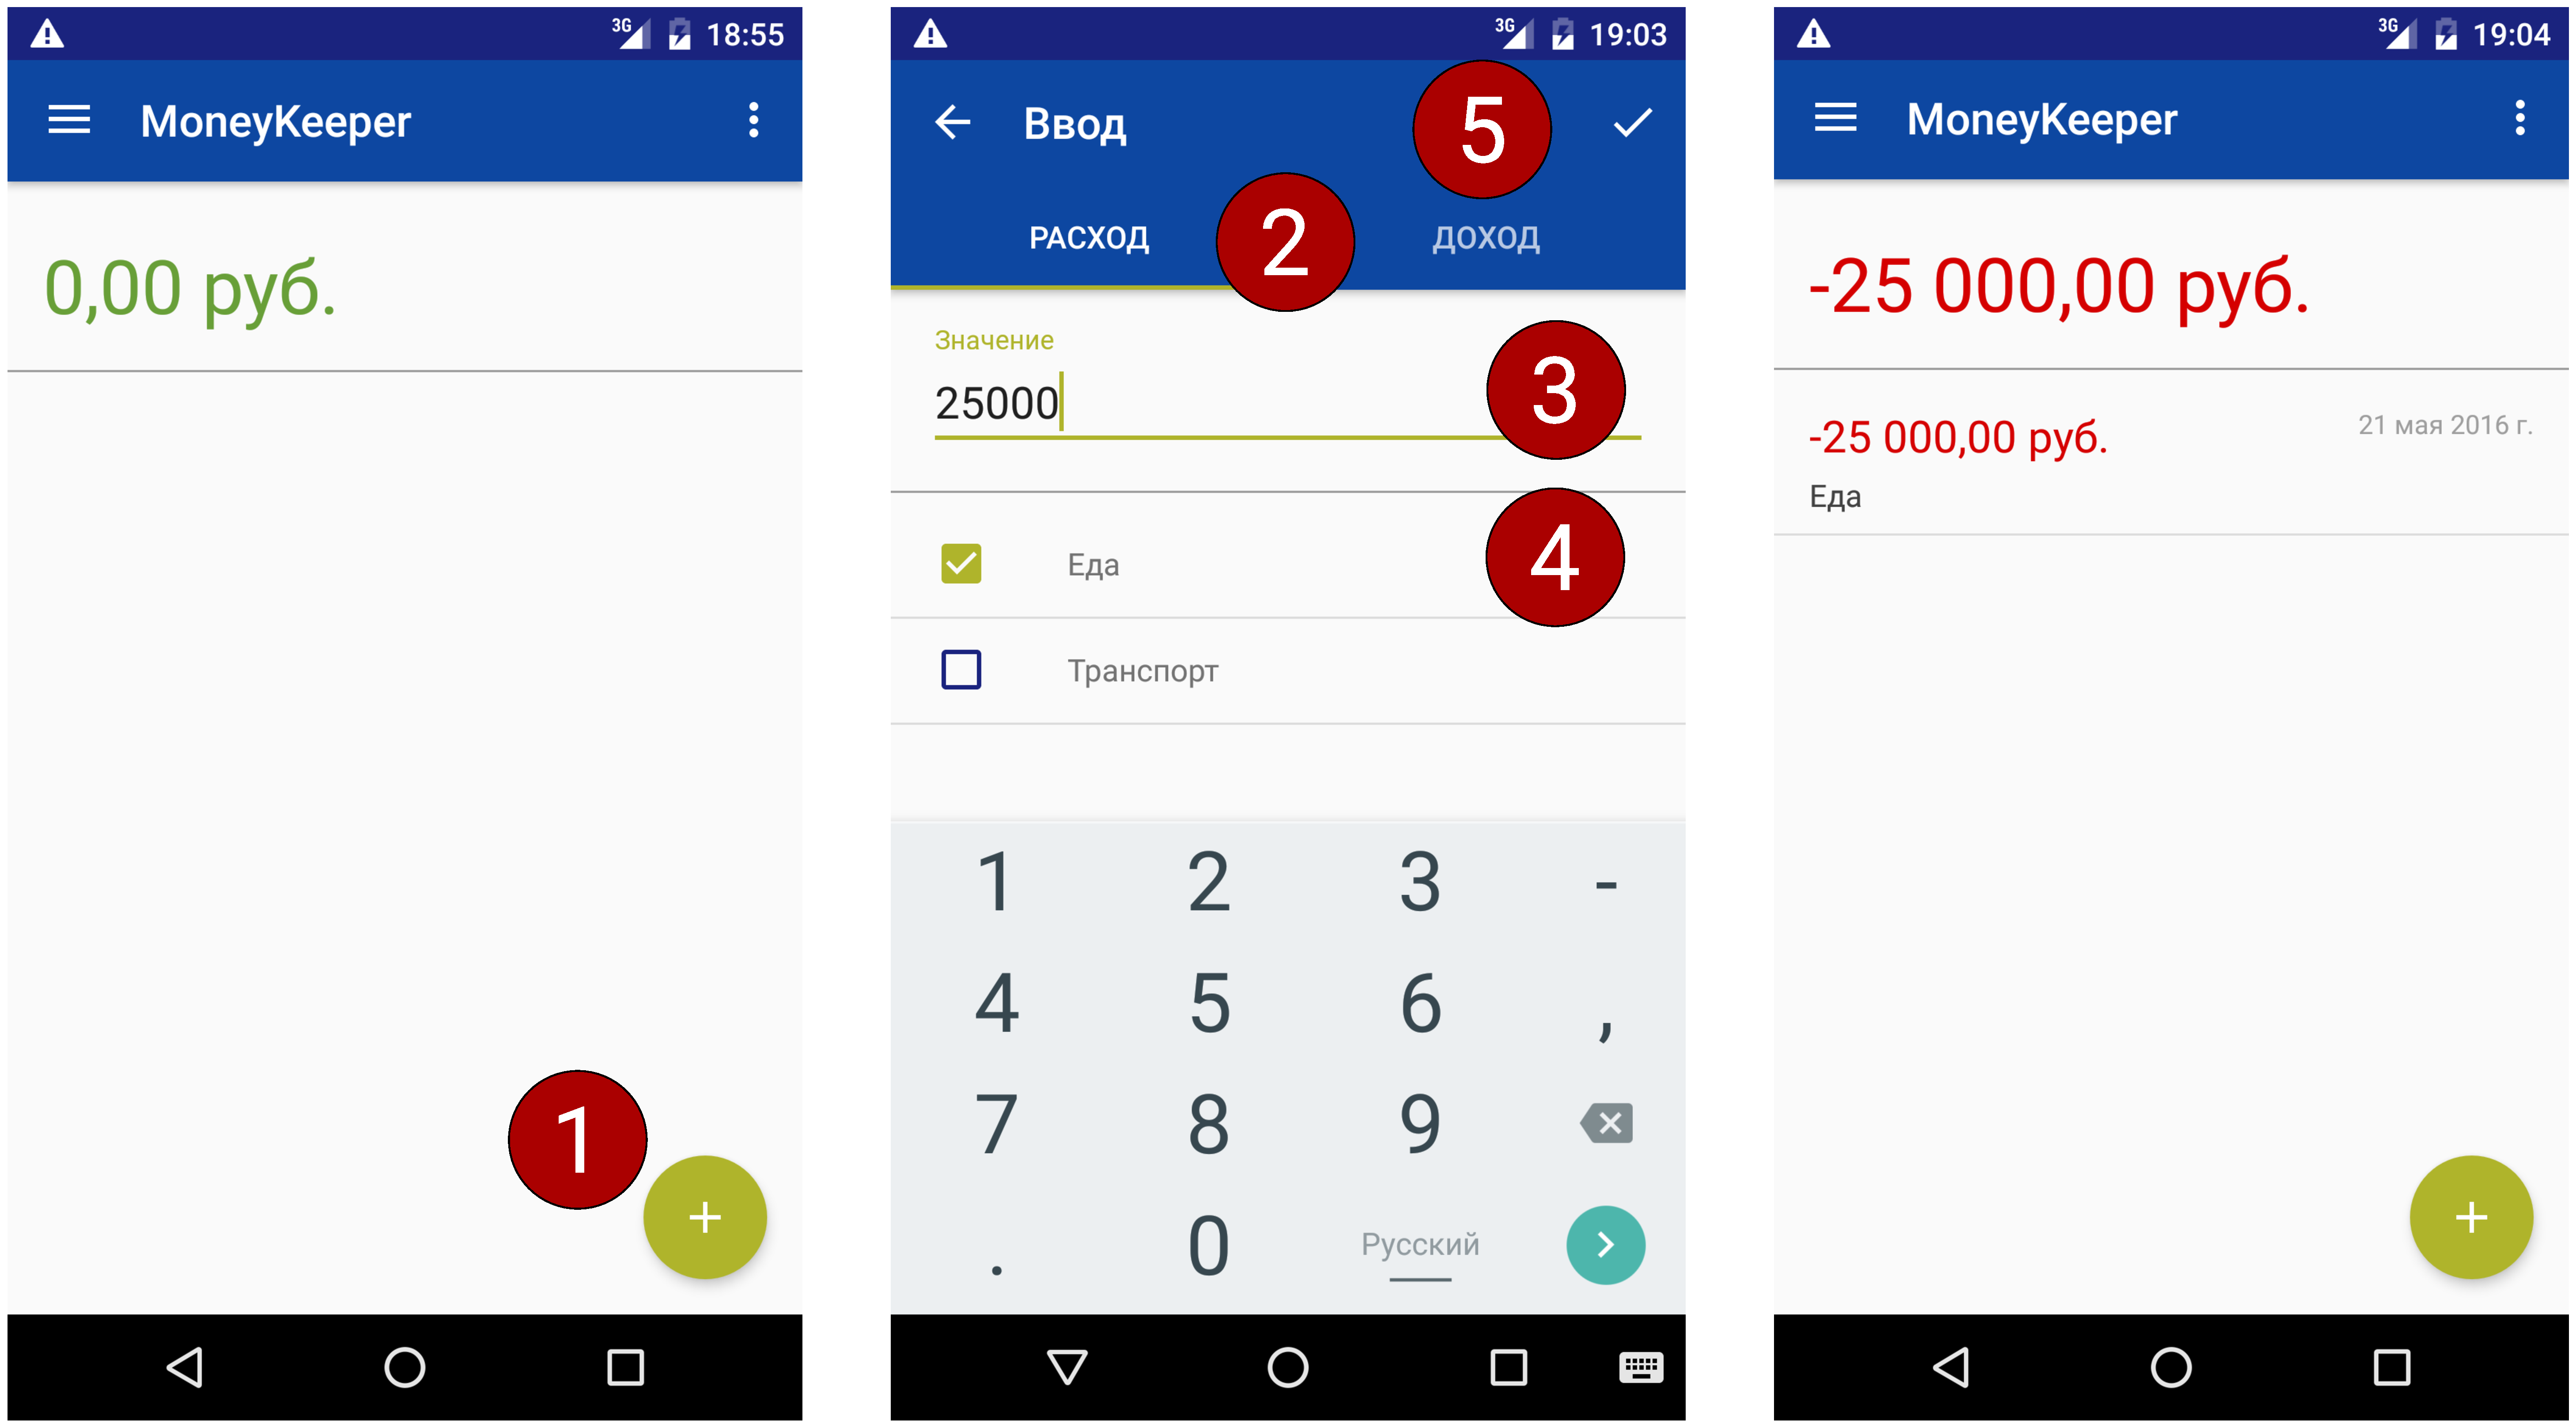
\includegraphics[width=140mm]{fig/implementation_manual_balance_change.eps}
  }
  \caption{Добавление изменения баланса}
  \label{fig:implementation_manual_balance_change}
\end{figure}

Редактирование данных выполняется подобным образом.
Основное отличие заключается в том, что для выполнения редактирования необходимо,
находясь на соответствующем экране просмотра,
выбрать требуемую запись, категорию учета или изменение баланса
путем нажатия на требуемый элемент списка.

Для того, чтобы удалить требуемое изменение баланса,
учетную запись или категорию учета, необходимо
выполнить сдвиг требуемого элемента списка на соответствующем экране просмотра.
При этом пользователю приложения предоставляется возможность отмены последнего
удаления путем нажатия на кнопку, расположенную в правом углу всплывающего
окна, показываемого после удаления.
Иллюстрация процесса удаления изменений баланса, учетных записей и категорий учета
представлена на рисунке~\ref{fig:implementation_manual_remove}.

\begin{figure}[h!]
  \centering
  \fcolorbox{gray}{white}{
    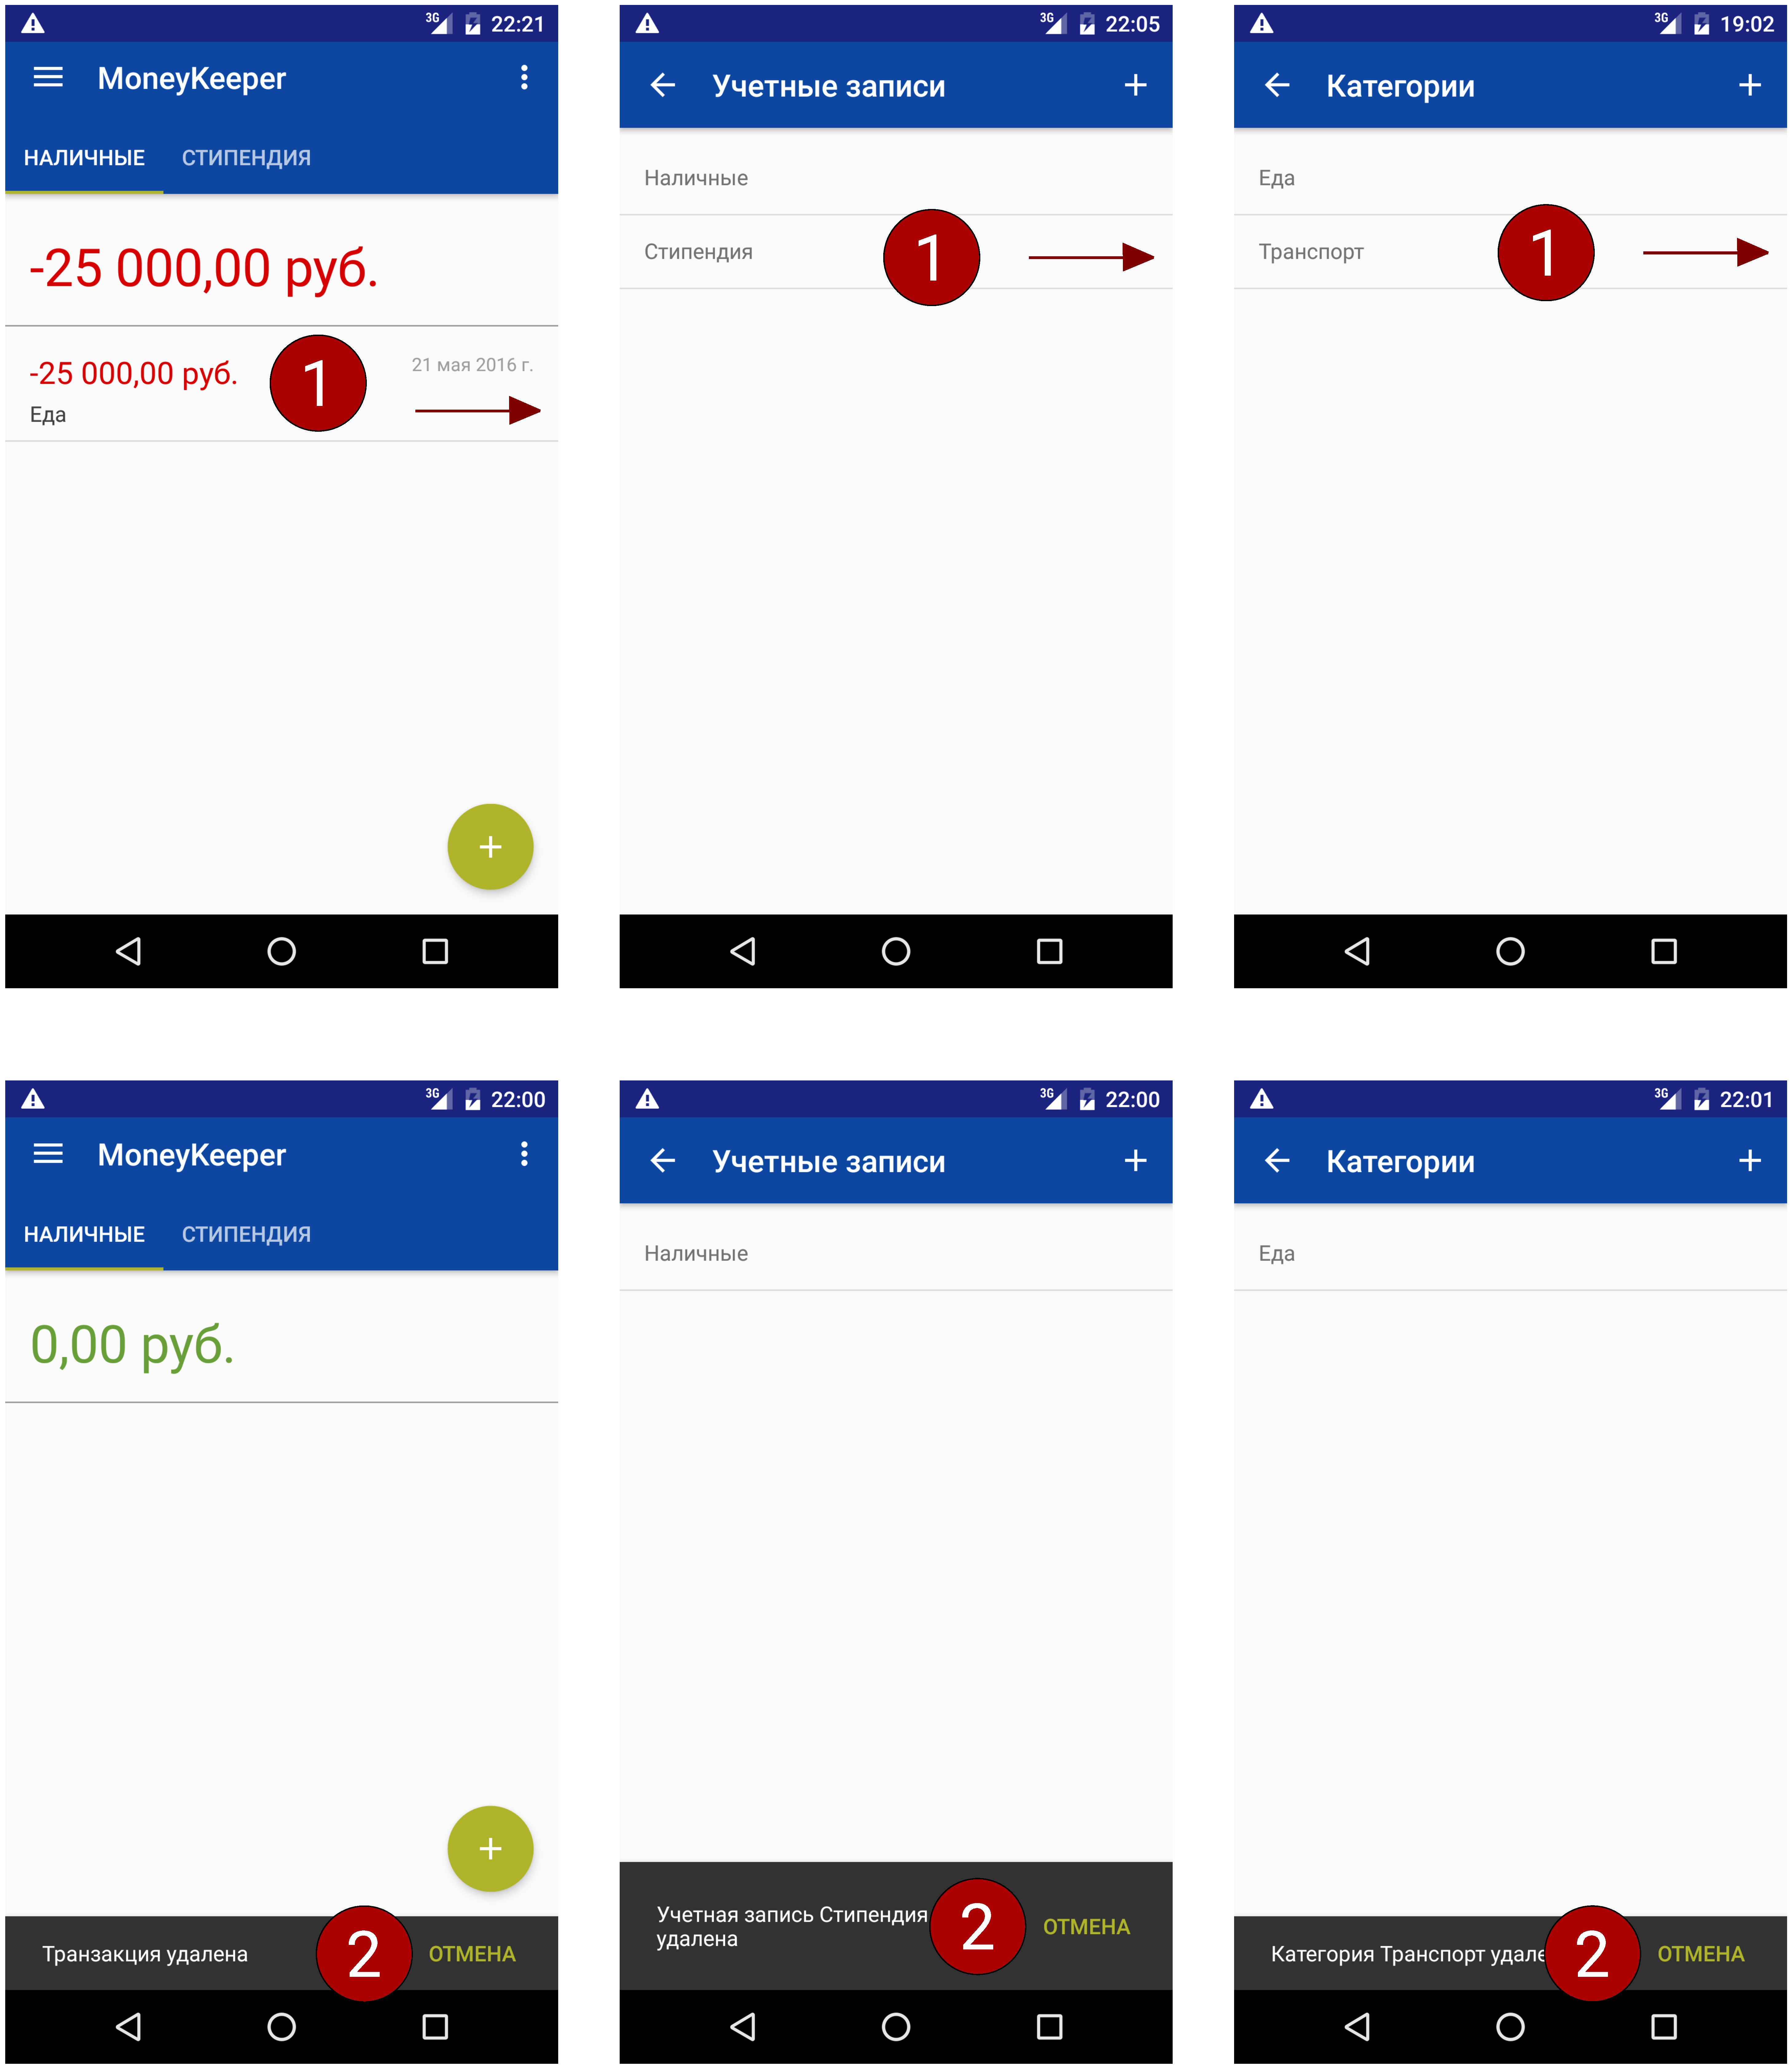
\includegraphics[width=140mm]{fig/implementation_manual_remove.eps}
  }
  \caption{Удаление данных}
  \label{fig:implementation_manual_remove}
\end{figure}

Отметим, что наряду с описанными, существует множество других вариантов
использования функциональности приложения.
Поскольку описание всех возможных сценариев заняло бы
чересчур много места, в данном подразделе были рассмотрены лишь базовые.
Благодаря унификации пользовательского интерфейса приложения
в соответствии с требованиями Material Design, данные сценарии представляются
интуитивно понятными и подобными друг другу.

\subsection{Перспективы развития}

Основными направлениеми развития всякого программного продукта является
добавление новой, а также развитие существующей функциональности.
В разрабатываемом приложении предпочтение отдается таким функциональным
возможностям, которые не усложняют пользовательский интерфейс.

На данный момент имеется два основных направления развития функциональности приложения.
Первая направление заключается в том, чтобы повысить точность распознавания величины
изменения баланса по изображению, получаемому с камеры мобильного устройства,
до такой степени, чтобы его можно было использовать в качестве основного механизма ввода.
Вторая направление предполагает использование алгоритмов машинного обучения
для сортировки категорий учета при вводе изменений баланса на основании
данных о местонахождения пользователя.
